\documentclass[]{article}
\usepackage{lmodern}
\usepackage{amssymb,amsmath}
\usepackage{ifxetex,ifluatex}
\usepackage{fixltx2e} % provides \textsubscript
\ifnum 0\ifxetex 1\fi\ifluatex 1\fi=0 % if pdftex
  \usepackage[T1]{fontenc}
  \usepackage[utf8]{inputenc}
\else % if luatex or xelatex
  \ifxetex
    \usepackage{mathspec}
  \else
    \usepackage{fontspec}
  \fi
  \defaultfontfeatures{Ligatures=TeX,Scale=MatchLowercase}
\fi
% use upquote if available, for straight quotes in verbatim environments
\IfFileExists{upquote.sty}{\usepackage{upquote}}{}
% use microtype if available
\IfFileExists{microtype.sty}{%
\usepackage{microtype}
\UseMicrotypeSet[protrusion]{basicmath} % disable protrusion for tt fonts
}{}
\usepackage[margin=1in]{geometry}
\usepackage{hyperref}
\hypersetup{unicode=true,
            pdftitle={A Very Extensive NCAA Exploratory Analysis},
            pdfauthor={Troy Walters},
            pdfborder={0 0 0},
            breaklinks=true}
\urlstyle{same}  % don't use monospace font for urls
\usepackage{color}
\usepackage{fancyvrb}
\newcommand{\VerbBar}{|}
\newcommand{\VERB}{\Verb[commandchars=\\\{\}]}
\DefineVerbatimEnvironment{Highlighting}{Verbatim}{commandchars=\\\{\}}
% Add ',fontsize=\small' for more characters per line
\usepackage{framed}
\definecolor{shadecolor}{RGB}{248,248,248}
\newenvironment{Shaded}{\begin{snugshade}}{\end{snugshade}}
\newcommand{\KeywordTok}[1]{\textcolor[rgb]{0.13,0.29,0.53}{\textbf{#1}}}
\newcommand{\DataTypeTok}[1]{\textcolor[rgb]{0.13,0.29,0.53}{#1}}
\newcommand{\DecValTok}[1]{\textcolor[rgb]{0.00,0.00,0.81}{#1}}
\newcommand{\BaseNTok}[1]{\textcolor[rgb]{0.00,0.00,0.81}{#1}}
\newcommand{\FloatTok}[1]{\textcolor[rgb]{0.00,0.00,0.81}{#1}}
\newcommand{\ConstantTok}[1]{\textcolor[rgb]{0.00,0.00,0.00}{#1}}
\newcommand{\CharTok}[1]{\textcolor[rgb]{0.31,0.60,0.02}{#1}}
\newcommand{\SpecialCharTok}[1]{\textcolor[rgb]{0.00,0.00,0.00}{#1}}
\newcommand{\StringTok}[1]{\textcolor[rgb]{0.31,0.60,0.02}{#1}}
\newcommand{\VerbatimStringTok}[1]{\textcolor[rgb]{0.31,0.60,0.02}{#1}}
\newcommand{\SpecialStringTok}[1]{\textcolor[rgb]{0.31,0.60,0.02}{#1}}
\newcommand{\ImportTok}[1]{#1}
\newcommand{\CommentTok}[1]{\textcolor[rgb]{0.56,0.35,0.01}{\textit{#1}}}
\newcommand{\DocumentationTok}[1]{\textcolor[rgb]{0.56,0.35,0.01}{\textbf{\textit{#1}}}}
\newcommand{\AnnotationTok}[1]{\textcolor[rgb]{0.56,0.35,0.01}{\textbf{\textit{#1}}}}
\newcommand{\CommentVarTok}[1]{\textcolor[rgb]{0.56,0.35,0.01}{\textbf{\textit{#1}}}}
\newcommand{\OtherTok}[1]{\textcolor[rgb]{0.56,0.35,0.01}{#1}}
\newcommand{\FunctionTok}[1]{\textcolor[rgb]{0.00,0.00,0.00}{#1}}
\newcommand{\VariableTok}[1]{\textcolor[rgb]{0.00,0.00,0.00}{#1}}
\newcommand{\ControlFlowTok}[1]{\textcolor[rgb]{0.13,0.29,0.53}{\textbf{#1}}}
\newcommand{\OperatorTok}[1]{\textcolor[rgb]{0.81,0.36,0.00}{\textbf{#1}}}
\newcommand{\BuiltInTok}[1]{#1}
\newcommand{\ExtensionTok}[1]{#1}
\newcommand{\PreprocessorTok}[1]{\textcolor[rgb]{0.56,0.35,0.01}{\textit{#1}}}
\newcommand{\AttributeTok}[1]{\textcolor[rgb]{0.77,0.63,0.00}{#1}}
\newcommand{\RegionMarkerTok}[1]{#1}
\newcommand{\InformationTok}[1]{\textcolor[rgb]{0.56,0.35,0.01}{\textbf{\textit{#1}}}}
\newcommand{\WarningTok}[1]{\textcolor[rgb]{0.56,0.35,0.01}{\textbf{\textit{#1}}}}
\newcommand{\AlertTok}[1]{\textcolor[rgb]{0.94,0.16,0.16}{#1}}
\newcommand{\ErrorTok}[1]{\textcolor[rgb]{0.64,0.00,0.00}{\textbf{#1}}}
\newcommand{\NormalTok}[1]{#1}
\usepackage{graphicx,grffile}
\makeatletter
\def\maxwidth{\ifdim\Gin@nat@width>\linewidth\linewidth\else\Gin@nat@width\fi}
\def\maxheight{\ifdim\Gin@nat@height>\textheight\textheight\else\Gin@nat@height\fi}
\makeatother
% Scale images if necessary, so that they will not overflow the page
% margins by default, and it is still possible to overwrite the defaults
% using explicit options in \includegraphics[width, height, ...]{}
\setkeys{Gin}{width=\maxwidth,height=\maxheight,keepaspectratio}
\IfFileExists{parskip.sty}{%
\usepackage{parskip}
}{% else
\setlength{\parindent}{0pt}
\setlength{\parskip}{6pt plus 2pt minus 1pt}
}
\setlength{\emergencystretch}{3em}  % prevent overfull lines
\providecommand{\tightlist}{%
  \setlength{\itemsep}{0pt}\setlength{\parskip}{0pt}}
\setcounter{secnumdepth}{0}
% Redefines (sub)paragraphs to behave more like sections
\ifx\paragraph\undefined\else
\let\oldparagraph\paragraph
\renewcommand{\paragraph}[1]{\oldparagraph{#1}\mbox{}}
\fi
\ifx\subparagraph\undefined\else
\let\oldsubparagraph\subparagraph
\renewcommand{\subparagraph}[1]{\oldsubparagraph{#1}\mbox{}}
\fi

%%% Use protect on footnotes to avoid problems with footnotes in titles
\let\rmarkdownfootnote\footnote%
\def\footnote{\protect\rmarkdownfootnote}

%%% Change title format to be more compact
\usepackage{titling}

% Create subtitle command for use in maketitle
\newcommand{\subtitle}[1]{
  \posttitle{
    \begin{center}\large#1\end{center}
    }
}

\setlength{\droptitle}{-2em}

  \title{A Very Extensive NCAA Exploratory Analysis}
    \pretitle{\vspace{\droptitle}\centering\huge}
  \posttitle{\par}
    \author{Troy Walters}
    \preauthor{\centering\large\emph}
  \postauthor{\par}
      \predate{\centering\large\emph}
  \postdate{\par}
    \date{February 20, 2018}


\begin{document}
\maketitle

\subsection{Libraries}\label{libraries}

\begin{Shaded}
\begin{Highlighting}[]
\KeywordTok{library}\NormalTok{(data.table)}
\KeywordTok{library}\NormalTok{(dplyr)}
\KeywordTok{library}\NormalTok{(magrittr)}
\KeywordTok{library}\NormalTok{(ggplot2)}
\KeywordTok{library}\NormalTok{(gridExtra)}
\KeywordTok{library}\NormalTok{(ggExtra)}
\KeywordTok{library}\NormalTok{(corrplot)}
\KeywordTok{library}\NormalTok{(factoextra)}
\KeywordTok{library}\NormalTok{(stringr)}
\KeywordTok{library}\NormalTok{(FactoMineR)}

\KeywordTok{theme_set}\NormalTok{(}\KeywordTok{theme_bw}\NormalTok{())}
\end{Highlighting}
\end{Shaded}

\begin{Shaded}
\begin{Highlighting}[]
\NormalTok{dir <-}\StringTok{ '/Users/JaviFerrando/Desktop/MLProject/input/'}
\KeywordTok{setwd}\NormalTok{(}\StringTok{"/Users/JaviFerrando/Desktop/MLProject"}\NormalTok{)}

\CommentTok{# Data Section 1}
\NormalTok{teams <-}\StringTok{ }\KeywordTok{fread}\NormalTok{(}\KeywordTok{paste}\NormalTok{(dir,}\StringTok{'Teams.csv'}\NormalTok{,}\DataTypeTok{sep=}\StringTok{''}\NormalTok{))}
\NormalTok{seasons <-}\StringTok{ }\KeywordTok{fread}\NormalTok{(}\KeywordTok{paste}\NormalTok{(dir,}\StringTok{'Seasons.csv'}\NormalTok{,}\DataTypeTok{sep=}\StringTok{''}\NormalTok{))}
\NormalTok{seeds <-}\StringTok{ }\KeywordTok{fread}\NormalTok{(}\KeywordTok{paste}\NormalTok{(dir,}\StringTok{'NCAATourneySeeds.csv'}\NormalTok{,}\DataTypeTok{sep=}\StringTok{''}\NormalTok{))}
\NormalTok{seas_results <-}\StringTok{ }\KeywordTok{fread}\NormalTok{(}\KeywordTok{paste}\NormalTok{(dir,}\StringTok{'RegularSeasonCompactResults.csv'}\NormalTok{,}\DataTypeTok{sep=}\StringTok{''}\NormalTok{))}
\NormalTok{tour_results <-}\StringTok{ }\KeywordTok{fread}\NormalTok{(}\KeywordTok{paste}\NormalTok{(dir,}\StringTok{'NCAATourneyCompactResults.csv'}\NormalTok{,}\DataTypeTok{sep=}\StringTok{''}\NormalTok{))}
\NormalTok{seas_detail <-}\StringTok{ }\KeywordTok{fread}\NormalTok{(}\KeywordTok{paste}\NormalTok{(dir,}\StringTok{'RegularSeasonDetailedResults.csv'}\NormalTok{,}\DataTypeTok{sep=}\StringTok{''}\NormalTok{))}
\NormalTok{tour_detail <-}\StringTok{ }\KeywordTok{fread}\NormalTok{(}\KeywordTok{paste}\NormalTok{(dir,}\StringTok{'NCAATourneyDetailedResults.csv'}\NormalTok{,}\DataTypeTok{sep=}\StringTok{''}\NormalTok{))}
\NormalTok{conferences <-}\StringTok{ }\KeywordTok{fread}\NormalTok{(}\KeywordTok{paste}\NormalTok{(dir,}\StringTok{'Conferences.csv'}\NormalTok{,}\DataTypeTok{sep=}\StringTok{''}\NormalTok{))}
\NormalTok{team_conferences <-}\StringTok{ }\KeywordTok{fread}\NormalTok{(}\KeywordTok{paste}\NormalTok{(dir,}\StringTok{'TeamConferences.csv'}\NormalTok{,}\DataTypeTok{sep=}\StringTok{''}\NormalTok{))}
\NormalTok{coaches <-}\StringTok{ }\KeywordTok{fread}\NormalTok{(}\KeywordTok{paste}\NormalTok{(dir,}\StringTok{'TeamCoaches.csv'}\NormalTok{,}\DataTypeTok{sep=}\StringTok{''}\NormalTok{))}
\NormalTok{tour_enrich <-}\StringTok{ }\KeywordTok{fread}\NormalTok{(}\KeywordTok{paste}\NormalTok{(dir,}\StringTok{'NCAATourneyDetailedResultsEnriched.csv'}\NormalTok{,}\DataTypeTok{sep=}\StringTok{''}\NormalTok{))}
\NormalTok{seas_enrich <-}\StringTok{ }\KeywordTok{fread}\NormalTok{(}\KeywordTok{paste}\NormalTok{(dir,}\StringTok{'NCAASeasonDetailedResultsEnriched.csv'}\NormalTok{,}\DataTypeTok{sep=}\StringTok{''}\NormalTok{))}
\end{Highlighting}
\end{Shaded}

\begin{Shaded}
\begin{Highlighting}[]
\KeywordTok{setkey}\NormalTok{(teams, TeamID)}
\KeywordTok{setkey}\NormalTok{(seeds, TeamID)}

\NormalTok{g1 <-}
\StringTok{    }\NormalTok{teams[seeds][, one_seed }\OperatorTok{:}\ErrorTok{=}\StringTok{ }\KeywordTok{as.numeric}\NormalTok{(}\KeywordTok{substr}\NormalTok{(Seed, }\DecValTok{2}\NormalTok{, }\DecValTok{3}\NormalTok{)) }\OperatorTok{==}\StringTok{ }\DecValTok{1}\NormalTok{][, }\KeywordTok{sum}\NormalTok{(one_seed), by =}\StringTok{ }\NormalTok{TeamName][}\KeywordTok{order}\NormalTok{(V1, }\DataTypeTok{decreasing =}\NormalTok{ T)][}\DecValTok{1}\OperatorTok{:}\DecValTok{15}\NormalTok{,] }\OperatorTok
\StringTok{    }\KeywordTok{ggplot}\NormalTok{(}\KeywordTok{aes}\NormalTok{(}\DataTypeTok{x =} \KeywordTok{reorder}\NormalTok{(TeamName, V1), }\DataTypeTok{y =}\NormalTok{ V1)) }\OperatorTok{+}
\StringTok{    }\KeywordTok{geom_bar}\NormalTok{(}\DataTypeTok{stat =} \StringTok{'identity'}\NormalTok{, }\DataTypeTok{fill =} \StringTok{'darkblue'}\NormalTok{) }\OperatorTok{+}
\StringTok{    }\KeywordTok{labs}\NormalTok{(}\DataTypeTok{x =} \StringTok{''}\NormalTok{, }\DataTypeTok{y =} \StringTok{'No 1 seeds'}\NormalTok{, }\DataTypeTok{title =} \StringTok{'No. 1 Seeds since 1985'}\NormalTok{) }\OperatorTok{+}
\StringTok{    }\KeywordTok{coord_flip}\NormalTok{()}

\KeywordTok{setkey}\NormalTok{(seas_results, WTeamID)}

\NormalTok{g2 <-}
\StringTok{    }\NormalTok{seas_results[teams][, .(}\DataTypeTok{wins =}\NormalTok{ .N), by =}\StringTok{ }\NormalTok{TeamName][}\KeywordTok{order}\NormalTok{(}\OperatorTok{-}\NormalTok{wins)][}\DecValTok{1}\OperatorTok{:}\DecValTok{15}\NormalTok{,] }\OperatorTok
\StringTok{    }\KeywordTok{ggplot}\NormalTok{(}\KeywordTok{aes}\NormalTok{(}\DataTypeTok{x =} \KeywordTok{reorder}\NormalTok{(TeamName, wins), }\DataTypeTok{y =}\NormalTok{ wins)) }\OperatorTok{+}
\StringTok{    }\KeywordTok{geom_bar}\NormalTok{(}\DataTypeTok{stat =} \StringTok{'identity'}\NormalTok{, }\DataTypeTok{fill =} \StringTok{'darkblue'}\NormalTok{) }\OperatorTok{+}
\StringTok{    }\KeywordTok{labs}\NormalTok{(}\DataTypeTok{x =} \StringTok{''}\NormalTok{, }\DataTypeTok{y =} \StringTok{'Wins'}\NormalTok{, }\DataTypeTok{title =} \StringTok{'Regular Season Wins since 1985'}\NormalTok{) }\OperatorTok{+}
\StringTok{    }\KeywordTok{coord_flip}\NormalTok{()}

\KeywordTok{setkey}\NormalTok{(tour_results, WTeamID)}

\NormalTok{g3 <-}
\StringTok{    }\NormalTok{tour_results[teams][, .(}\DataTypeTok{wins =}\NormalTok{ .N), by =}\StringTok{ }\NormalTok{TeamName][}\KeywordTok{order}\NormalTok{(}\OperatorTok{-}\NormalTok{wins)][}\DecValTok{1}\OperatorTok{:}\DecValTok{15}\NormalTok{,] }\OperatorTok
\StringTok{    }\KeywordTok{ggplot}\NormalTok{(}\KeywordTok{aes}\NormalTok{(}\DataTypeTok{x =} \KeywordTok{reorder}\NormalTok{(TeamName, wins), }\DataTypeTok{y =}\NormalTok{ wins)) }\OperatorTok{+}
\StringTok{    }\KeywordTok{geom_bar}\NormalTok{(}\DataTypeTok{stat =} \StringTok{'identity'}\NormalTok{, }\DataTypeTok{fill =} \StringTok{'darkblue'}\NormalTok{) }\OperatorTok{+}
\StringTok{    }\KeywordTok{labs}\NormalTok{(}\DataTypeTok{x =} \StringTok{''}\NormalTok{, }\DataTypeTok{y =} \StringTok{'Wins'}\NormalTok{, }\DataTypeTok{title =} \StringTok{'Tournament Wins since 1985'}\NormalTok{) }\OperatorTok{+}
\StringTok{    }\KeywordTok{coord_flip}\NormalTok{()}

\NormalTok{g4 <-}
\StringTok{    }\NormalTok{tour_results[teams][DayNum }\OperatorTok{==}\StringTok{ }\DecValTok{154}\NormalTok{, .(}\DataTypeTok{wins =}\NormalTok{ .N), by =}\StringTok{ }\NormalTok{TeamName][}\KeywordTok{order}\NormalTok{(}\OperatorTok{-}\NormalTok{wins)][}\DecValTok{1}\OperatorTok{:}\DecValTok{15}\NormalTok{,] }\OperatorTok
\StringTok{    }\KeywordTok{ggplot}\NormalTok{(}\KeywordTok{aes}\NormalTok{(}\DataTypeTok{x =} \KeywordTok{reorder}\NormalTok{(TeamName, wins), }\DataTypeTok{y =}\NormalTok{ wins)) }\OperatorTok{+}
\StringTok{    }\KeywordTok{geom_bar}\NormalTok{(}\DataTypeTok{stat =} \StringTok{'identity'}\NormalTok{, }\DataTypeTok{fill =} \StringTok{'darkblue'}\NormalTok{) }\OperatorTok{+}
\StringTok{    }\KeywordTok{labs}\NormalTok{(}\DataTypeTok{x =} \StringTok{''}\NormalTok{, }\DataTypeTok{y =} \StringTok{'Championships'}\NormalTok{, }\DataTypeTok{title =} \StringTok{'Tournament Championships since 1985'}\NormalTok{) }\OperatorTok{+}
\StringTok{    }\KeywordTok{coord_flip}\NormalTok{()}

\KeywordTok{grid.arrange}\NormalTok{(g1, g2, g3, g4, }\DataTypeTok{nrow =} \DecValTok{2}\NormalTok{)}
\end{Highlighting}
\end{Shaded}

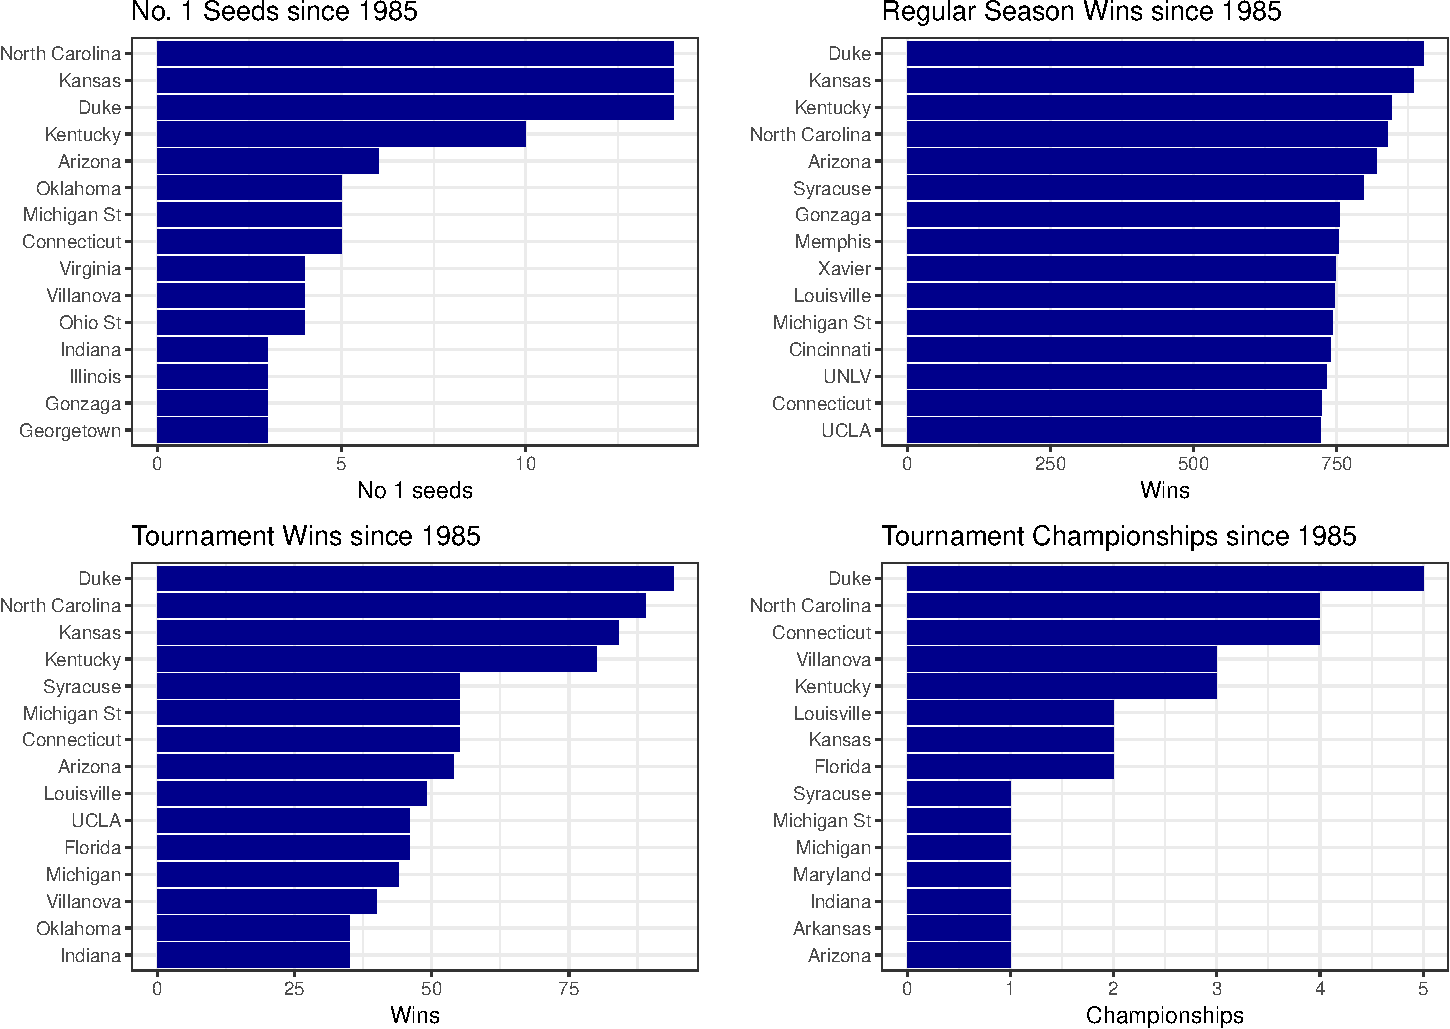
\includegraphics{EDA_files/figure-latex/unnamed-chunk-3-1.pdf} \#\#
Historical Performance \{\#historical\}

\subsection{Indicators of Regular Season Success}\label{regseason}

Let's now turn to the regular season game statistics. We are interested
in knowing how certain statistics correlate with winning vs losing. We
will take the regular season detail and first convert it to a more
`long' format with only 1 column of TeamIDs and a factor indicating
whether that row corresponds to a win or a loss. Here I also add some
additional game statistcs. These include field goal percentage, free
throw percentage, offensive/defensive rebounding efficiency, and
possessions. These last two come from Laksan Nathan's kernel
\href{https://www.kaggle.com/lnatml/feature-engineering-with-advanced-stats}{here}.

\begin{Shaded}
\begin{Highlighting}[]
\NormalTok{win_stats <-}\StringTok{ }\NormalTok{seas_enrich[, .(}
\NormalTok{    Season,}
    \DataTypeTok{TeamID =}\NormalTok{ WTeamID,}
    \DataTypeTok{Result =} \KeywordTok{rep}\NormalTok{(}\StringTok{'W'}\NormalTok{, .N),}
    \DataTypeTok{FGM =}\NormalTok{ WFGM,}
    \DataTypeTok{FGA =}\NormalTok{ WFGA,}
    \DataTypeTok{FGP =}\NormalTok{ WFGM }\OperatorTok{/}\StringTok{ }\NormalTok{WFGA,}
    \DataTypeTok{FGP2 =}\NormalTok{ (WFGM }\OperatorTok{-}\StringTok{ }\NormalTok{WFGM3) }\OperatorTok{/}\StringTok{ }\NormalTok{(WFGA }\OperatorTok{-}\StringTok{ }\NormalTok{WFGA3),}
    \DataTypeTok{FGM3 =}\NormalTok{ WFGM3,}
    \DataTypeTok{FGA3 =}\NormalTok{ WFGA3,}
    \DataTypeTok{FGP3 =}\NormalTok{ WFGM3 }\OperatorTok{/}\StringTok{ }\NormalTok{WFGA3,}
    \DataTypeTok{FTM =}\NormalTok{ WFTM,}
    \DataTypeTok{FTA =}\NormalTok{ WFTA,}
    \DataTypeTok{FTP =}\NormalTok{ WFTM }\OperatorTok{/}\StringTok{ }\NormalTok{WFTA,}
    \DataTypeTok{OR =}\NormalTok{ WOR,}
    \DataTypeTok{DR =}\NormalTok{ WDR,}
    \DataTypeTok{AST =}\NormalTok{ WAst,}
    \DataTypeTok{TO =}\NormalTok{ WTO,}
    \DataTypeTok{STL =}\NormalTok{ WStl,}
    \DataTypeTok{BLK =}\NormalTok{ WBlk,}
    \DataTypeTok{PF =}\NormalTok{ WPF,}
    \DataTypeTok{PIE =}\NormalTok{ WPIE,}
    \DataTypeTok{ORP =}\NormalTok{ WOR }\OperatorTok{/}\StringTok{ }\NormalTok{(WOR }\OperatorTok{+}\StringTok{ }\NormalTok{LDR),}
    \DataTypeTok{DRP =}\NormalTok{ WDR }\OperatorTok{/}\StringTok{ }\NormalTok{(WDR }\OperatorTok{+}\StringTok{ }\NormalTok{LOR),}
    \DataTypeTok{eFG =}\NormalTok{ WeFGP,}
    \DataTypeTok{NetRTG =}\NormalTok{ WNetRtg,}
    \DataTypeTok{FTAR =}\NormalTok{ WFTAR,}
    \DataTypeTok{POS =} \FloatTok{0.96} \OperatorTok{*}\StringTok{ }\NormalTok{(WFGA }\OperatorTok{+}\StringTok{ }\NormalTok{WTO }\OperatorTok{+}\StringTok{ }\FloatTok{0.44} \OperatorTok{*}\StringTok{ }\NormalTok{WFTA }\OperatorTok{-}\StringTok{ }\NormalTok{WOR)}
\NormalTok{    )]}

\NormalTok{los_stats <-}\StringTok{ }\NormalTok{seas_enrich[, .(}
\NormalTok{    Season,}
    \DataTypeTok{TeamID =}\NormalTok{ LTeamID,}
    \DataTypeTok{Result =} \KeywordTok{rep}\NormalTok{(}\StringTok{'L'}\NormalTok{, .N),}
    \DataTypeTok{FGM =}\NormalTok{ LFGM,}
    \DataTypeTok{FGA =}\NormalTok{ LFGA,}
    \DataTypeTok{FGP =}\NormalTok{ LFGM }\OperatorTok{/}\StringTok{ }\NormalTok{LFGA,}
    \DataTypeTok{FGP2 =}\NormalTok{ (LFGM }\OperatorTok{-}\StringTok{ }\NormalTok{LFGM3) }\OperatorTok{/}\StringTok{ }\NormalTok{(LFGA }\OperatorTok{-}\StringTok{ }\NormalTok{LFGA3),}
    \DataTypeTok{FGM3 =}\NormalTok{ LFGM3,}
    \DataTypeTok{FGA3 =}\NormalTok{ LFGA3,}
    \DataTypeTok{FGP3 =}\NormalTok{ LFGM3 }\OperatorTok{/}\StringTok{ }\NormalTok{LFGA3,}
    \DataTypeTok{FTM =}\NormalTok{ LFTM,}
    \DataTypeTok{FTA =}\NormalTok{ LFTA,}
    \DataTypeTok{FTP =}\NormalTok{ LFTM }\OperatorTok{/}\StringTok{ }\NormalTok{LFTA,}
    \DataTypeTok{OR =}\NormalTok{ LOR,}
    \DataTypeTok{DR =}\NormalTok{ LDR,}
    \DataTypeTok{AST =}\NormalTok{ LAst,}
    \DataTypeTok{TO =}\NormalTok{ LTO,}
    \DataTypeTok{STL =}\NormalTok{ LStl,}
    \DataTypeTok{BLK =}\NormalTok{ LBlk,}
    \DataTypeTok{PF =}\NormalTok{ LPF,}
    \DataTypeTok{PIE =}\NormalTok{ LPIE,}
    \DataTypeTok{ORP =}\NormalTok{ (LOR }\OperatorTok{/}\StringTok{ }\NormalTok{(LOR }\OperatorTok{+}\StringTok{ }\NormalTok{WDR)),}
    \DataTypeTok{DRP =}\NormalTok{ LDR }\OperatorTok{/}\StringTok{ }\NormalTok{(LDR }\OperatorTok{+}\StringTok{ }\NormalTok{WOR),}
    \DataTypeTok{eFG =}\NormalTok{ LeFGP,}
    \DataTypeTok{NetRTG =}\NormalTok{ LNetRtg,}
    \DataTypeTok{FTAR =}\NormalTok{ LFTAR,}
    \DataTypeTok{POS =} \FloatTok{0.96} \OperatorTok{*}\StringTok{ }\NormalTok{(LFGA }\OperatorTok{+}\StringTok{ }\NormalTok{LTO }\OperatorTok{+}\StringTok{ }\FloatTok{0.44} \OperatorTok{*}\StringTok{ }\NormalTok{LFTA }\OperatorTok{-}\StringTok{ }\NormalTok{LOR)}
\NormalTok{    )]}

\NormalTok{stats_all <-}\StringTok{ }\KeywordTok{rbindlist}\NormalTok{(}\KeywordTok{list}\NormalTok{(win_stats, los_stats))}
\end{Highlighting}
\end{Shaded}

Now let's take a look at the distributions of these statistics for
winning and losing teams.

\begin{Shaded}
\begin{Highlighting}[]
\NormalTok{g1 <-}\StringTok{ }\NormalTok{stats_all }\OperatorTok
\StringTok{    }\KeywordTok{ggplot}\NormalTok{(}\KeywordTok{aes}\NormalTok{(}\DataTypeTok{x =}\NormalTok{ FGP, }\DataTypeTok{fill =}\NormalTok{ Result)) }\OperatorTok{+}
\StringTok{    }\KeywordTok{geom_density}\NormalTok{(}\DataTypeTok{alpha =} \FloatTok{0.6}\NormalTok{) }\OperatorTok{+}
\StringTok{    }\KeywordTok{scale_fill_manual}\NormalTok{(}\DataTypeTok{values =} \KeywordTok{c}\NormalTok{(}\StringTok{'#FF6666'}\NormalTok{, }\StringTok{'#33FF00'}\NormalTok{)) }\OperatorTok{+}\StringTok{ }
\StringTok{    }\KeywordTok{labs}\NormalTok{(}\DataTypeTok{x =} \StringTok{'Field Goals %'}\NormalTok{, }\DataTypeTok{y =} \StringTok{''}\NormalTok{, }\DataTypeTok{title =} \StringTok{'Field Goal M/A Ratio'}\NormalTok{)}

\NormalTok{g2 <-}\StringTok{ }\NormalTok{stats_all }\OperatorTok
\StringTok{    }\KeywordTok{ggplot}\NormalTok{(}\KeywordTok{aes}\NormalTok{(}\DataTypeTok{x =}\NormalTok{ FGP2, }\DataTypeTok{fill =}\NormalTok{ Result)) }\OperatorTok{+}
\StringTok{    }\KeywordTok{geom_density}\NormalTok{(}\DataTypeTok{alpha =} \FloatTok{0.6}\NormalTok{) }\OperatorTok{+}
\StringTok{    }\KeywordTok{scale_fill_manual}\NormalTok{(}\DataTypeTok{values =} \KeywordTok{c}\NormalTok{(}\StringTok{'#FF6666'}\NormalTok{, }\StringTok{'#33FF00'}\NormalTok{)) }\OperatorTok{+}\StringTok{ }
\StringTok{    }\KeywordTok{labs}\NormalTok{(}\DataTypeTok{x =} \StringTok{'2-pt Field Goal %'}\NormalTok{, }\DataTypeTok{y =} \StringTok{''}\NormalTok{, }\DataTypeTok{title =} \StringTok{'2 Pt Field Goals M/A Ratio'}\NormalTok{)}

\NormalTok{g3 <-}\StringTok{ }\NormalTok{stats_all }\OperatorTok
\StringTok{    }\KeywordTok{ggplot}\NormalTok{(}\KeywordTok{aes}\NormalTok{(}\DataTypeTok{x =}\NormalTok{ FGP3, }\DataTypeTok{fill =}\NormalTok{ Result)) }\OperatorTok{+}
\StringTok{    }\KeywordTok{geom_density}\NormalTok{(}\DataTypeTok{alpha =} \FloatTok{0.6}\NormalTok{) }\OperatorTok{+}
\StringTok{    }\KeywordTok{scale_fill_manual}\NormalTok{(}\DataTypeTok{values =} \KeywordTok{c}\NormalTok{(}\StringTok{'#FF6666'}\NormalTok{, }\StringTok{'#33FF00'}\NormalTok{)) }\OperatorTok{+}\StringTok{ }
\StringTok{    }\KeywordTok{labs}\NormalTok{(}\DataTypeTok{x =} \StringTok{'3-pt Field Goal %'}\NormalTok{, }\DataTypeTok{y =} \StringTok{''}\NormalTok{, }\DataTypeTok{title =} \StringTok{'3 Pt Field Goals M/A Ratio'}\NormalTok{)}

\NormalTok{g4 <-}\StringTok{ }\NormalTok{stats_all }\OperatorTok
\StringTok{    }\KeywordTok{ggplot}\NormalTok{(}\KeywordTok{aes}\NormalTok{(}\DataTypeTok{x =}\NormalTok{ FTP, }\DataTypeTok{fill =}\NormalTok{ Result)) }\OperatorTok{+}
\StringTok{    }\KeywordTok{geom_density}\NormalTok{(}\DataTypeTok{alpha =} \FloatTok{0.6}\NormalTok{) }\OperatorTok{+}
\StringTok{    }\KeywordTok{scale_fill_manual}\NormalTok{(}\DataTypeTok{values =} \KeywordTok{c}\NormalTok{(}\StringTok{'#FF6666'}\NormalTok{, }\StringTok{'#33FF00'}\NormalTok{)) }\OperatorTok{+}\StringTok{ }
\StringTok{    }\KeywordTok{labs}\NormalTok{(}\DataTypeTok{x =} \StringTok{'Free Throw %'}\NormalTok{, }\DataTypeTok{y =} \StringTok{''}\NormalTok{, }\DataTypeTok{title =} \StringTok{'Free Throw Goals M/A Ratio'}\NormalTok{)}


\KeywordTok{grid.arrange}\NormalTok{(g1, g3, g4, }\DataTypeTok{ncol =} \DecValTok{3}\NormalTok{)}
\end{Highlighting}
\end{Shaded}

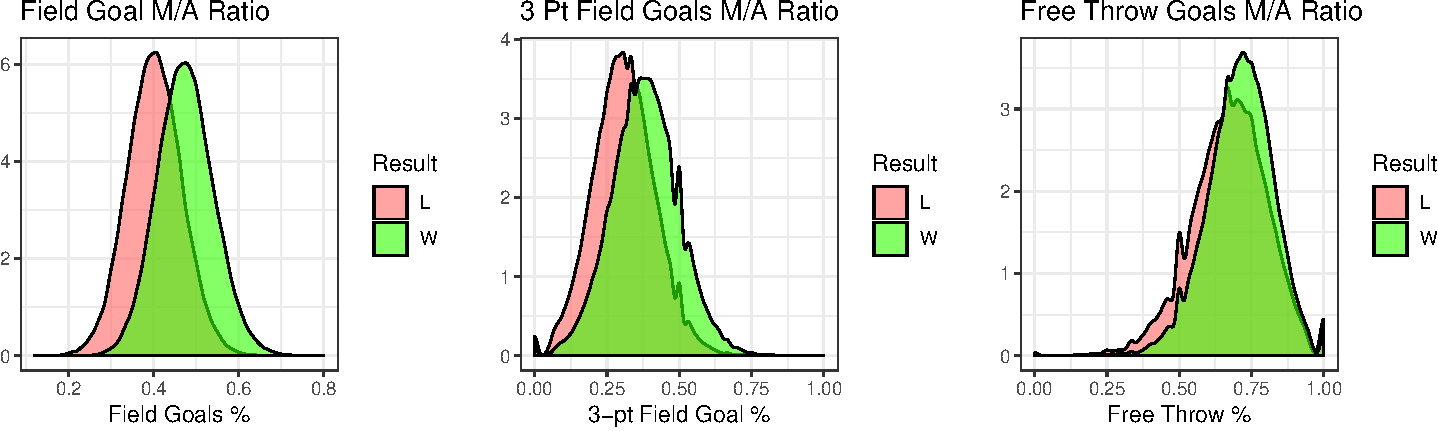
\includegraphics{EDA_files/figure-latex/unnamed-chunk-5-1.pdf}

\begin{Shaded}
\begin{Highlighting}[]
\NormalTok{g5 <-}\StringTok{ }\NormalTok{stats_all }\OperatorTok
\StringTok{    }\KeywordTok{ggplot}\NormalTok{(}\KeywordTok{aes}\NormalTok{(}\DataTypeTok{x =}\NormalTok{ OR, }\DataTypeTok{fill =}\NormalTok{ Result)) }\OperatorTok{+}
\StringTok{    }\KeywordTok{geom_density}\NormalTok{(}\DataTypeTok{alpha =} \FloatTok{0.6}\NormalTok{) }\OperatorTok{+}
\StringTok{    }\KeywordTok{scale_fill_manual}\NormalTok{(}\DataTypeTok{values =} \KeywordTok{c}\NormalTok{(}\StringTok{'#FF6666'}\NormalTok{, }\StringTok{'#66FF33'}\NormalTok{)) }\OperatorTok{+}\StringTok{ }
\StringTok{    }\KeywordTok{labs}\NormalTok{(}\DataTypeTok{x =} \StringTok{'Number of Offensive rebounds'}\NormalTok{, }\DataTypeTok{y =} \StringTok{''}\NormalTok{, }\DataTypeTok{title =} \StringTok{'Offensive Rebounds'}\NormalTok{)}

\NormalTok{g6 <-}\StringTok{ }\NormalTok{stats_all }\OperatorTok
\StringTok{    }\KeywordTok{ggplot}\NormalTok{(}\KeywordTok{aes}\NormalTok{(}\DataTypeTok{x =}\NormalTok{ DR, }\DataTypeTok{fill =}\NormalTok{ Result)) }\OperatorTok{+}
\StringTok{    }\KeywordTok{geom_density}\NormalTok{(}\DataTypeTok{alpha =} \FloatTok{0.6}\NormalTok{) }\OperatorTok{+}
\StringTok{    }\KeywordTok{scale_fill_manual}\NormalTok{(}\DataTypeTok{values =} \KeywordTok{c}\NormalTok{(}\StringTok{'#FF6666'}\NormalTok{, }\StringTok{'#66FF33'}\NormalTok{)) }\OperatorTok{+}\StringTok{ }
\StringTok{    }\KeywordTok{labs}\NormalTok{(}\DataTypeTok{x =} \StringTok{'Number of Defensive rebounds'}\NormalTok{, }\DataTypeTok{y =} \StringTok{''}\NormalTok{, }\DataTypeTok{title =} \StringTok{'Defensive Rebounds'}\NormalTok{)}

\NormalTok{g7 <-}\StringTok{ }\NormalTok{stats_all }\OperatorTok
\StringTok{    }\KeywordTok{ggplot}\NormalTok{(}\KeywordTok{aes}\NormalTok{(}\DataTypeTok{x =}\NormalTok{ AST, }\DataTypeTok{fill =}\NormalTok{ Result)) }\OperatorTok{+}
\StringTok{    }\KeywordTok{geom_density}\NormalTok{(}\DataTypeTok{alpha =} \FloatTok{0.6}\NormalTok{) }\OperatorTok{+}
\StringTok{    }\KeywordTok{scale_fill_manual}\NormalTok{(}\DataTypeTok{values =} \KeywordTok{c}\NormalTok{(}\StringTok{'#FF6666'}\NormalTok{, }\StringTok{'#66FF33'}\NormalTok{)) }\OperatorTok{+}\StringTok{ }
\StringTok{    }\KeywordTok{labs}\NormalTok{(}\DataTypeTok{x =} \StringTok{'Assists'}\NormalTok{, }\DataTypeTok{y =} \StringTok{''}\NormalTok{, }\DataTypeTok{title =} \StringTok{'Number of assists'}\NormalTok{)}

\NormalTok{g8 <-}\StringTok{ }\NormalTok{stats_all }\OperatorTok
\StringTok{    }\KeywordTok{ggplot}\NormalTok{(}\KeywordTok{aes}\NormalTok{(}\DataTypeTok{x =}\NormalTok{ TO, }\DataTypeTok{fill =}\NormalTok{ Result)) }\OperatorTok{+}
\StringTok{    }\KeywordTok{geom_density}\NormalTok{(}\DataTypeTok{alpha =} \FloatTok{0.6}\NormalTok{) }\OperatorTok{+}
\StringTok{    }\KeywordTok{scale_fill_manual}\NormalTok{(}\DataTypeTok{values =} \KeywordTok{c}\NormalTok{(}\StringTok{'#FF6666'}\NormalTok{, }\StringTok{'#66FF33'}\NormalTok{)) }\OperatorTok{+}\StringTok{ }
\StringTok{    }\KeywordTok{labs}\NormalTok{(}\DataTypeTok{x =} \StringTok{'Turnovers'}\NormalTok{, }\DataTypeTok{y =} \StringTok{''}\NormalTok{, }\DataTypeTok{title =} \StringTok{'Number of turnovers'}\NormalTok{)}

\NormalTok{g9 <-}\StringTok{ }\NormalTok{stats_all }\OperatorTok
\StringTok{    }\KeywordTok{ggplot}\NormalTok{(}\KeywordTok{aes}\NormalTok{(}\DataTypeTok{x =}\NormalTok{ STL, }\DataTypeTok{fill =}\NormalTok{ Result)) }\OperatorTok{+}
\StringTok{    }\KeywordTok{geom_density}\NormalTok{(}\DataTypeTok{alpha =} \FloatTok{0.6}\NormalTok{) }\OperatorTok{+}
\StringTok{    }\KeywordTok{scale_fill_manual}\NormalTok{(}\DataTypeTok{values =} \KeywordTok{c}\NormalTok{(}\StringTok{'#FF6666'}\NormalTok{, }\StringTok{'#66FF33'}\NormalTok{)) }\OperatorTok{+}\StringTok{ }
\StringTok{    }\KeywordTok{labs}\NormalTok{(}\DataTypeTok{x =} \StringTok{'Steals'}\NormalTok{, }\DataTypeTok{y =} \StringTok{''}\NormalTok{, }\DataTypeTok{title =} \StringTok{'Steals per Game'}\NormalTok{)}

\NormalTok{g10 <-}\StringTok{ }\NormalTok{stats_all }\OperatorTok
\StringTok{    }\KeywordTok{ggplot}\NormalTok{(}\KeywordTok{aes}\NormalTok{(}\DataTypeTok{x =}\NormalTok{ BLK, }\DataTypeTok{fill =}\NormalTok{ Result)) }\OperatorTok{+}
\StringTok{    }\KeywordTok{geom_density}\NormalTok{(}\DataTypeTok{alpha =} \FloatTok{0.6}\NormalTok{) }\OperatorTok{+}
\StringTok{    }\KeywordTok{scale_fill_manual}\NormalTok{(}\DataTypeTok{values =} \KeywordTok{c}\NormalTok{(}\StringTok{'#FF6666'}\NormalTok{, }\StringTok{'#66FF33'}\NormalTok{)) }\OperatorTok{+}\StringTok{ }
\StringTok{    }\KeywordTok{labs}\NormalTok{(}\DataTypeTok{x =} \StringTok{'Blocks'}\NormalTok{, }\DataTypeTok{y =} \StringTok{''}\NormalTok{, }\DataTypeTok{title =} \StringTok{'Blocks per Game'}\NormalTok{)}

\KeywordTok{grid.arrange}\NormalTok{(g5, g6, g7, g8, }\DataTypeTok{ncol =} \DecValTok{2}\NormalTok{)}
\end{Highlighting}
\end{Shaded}

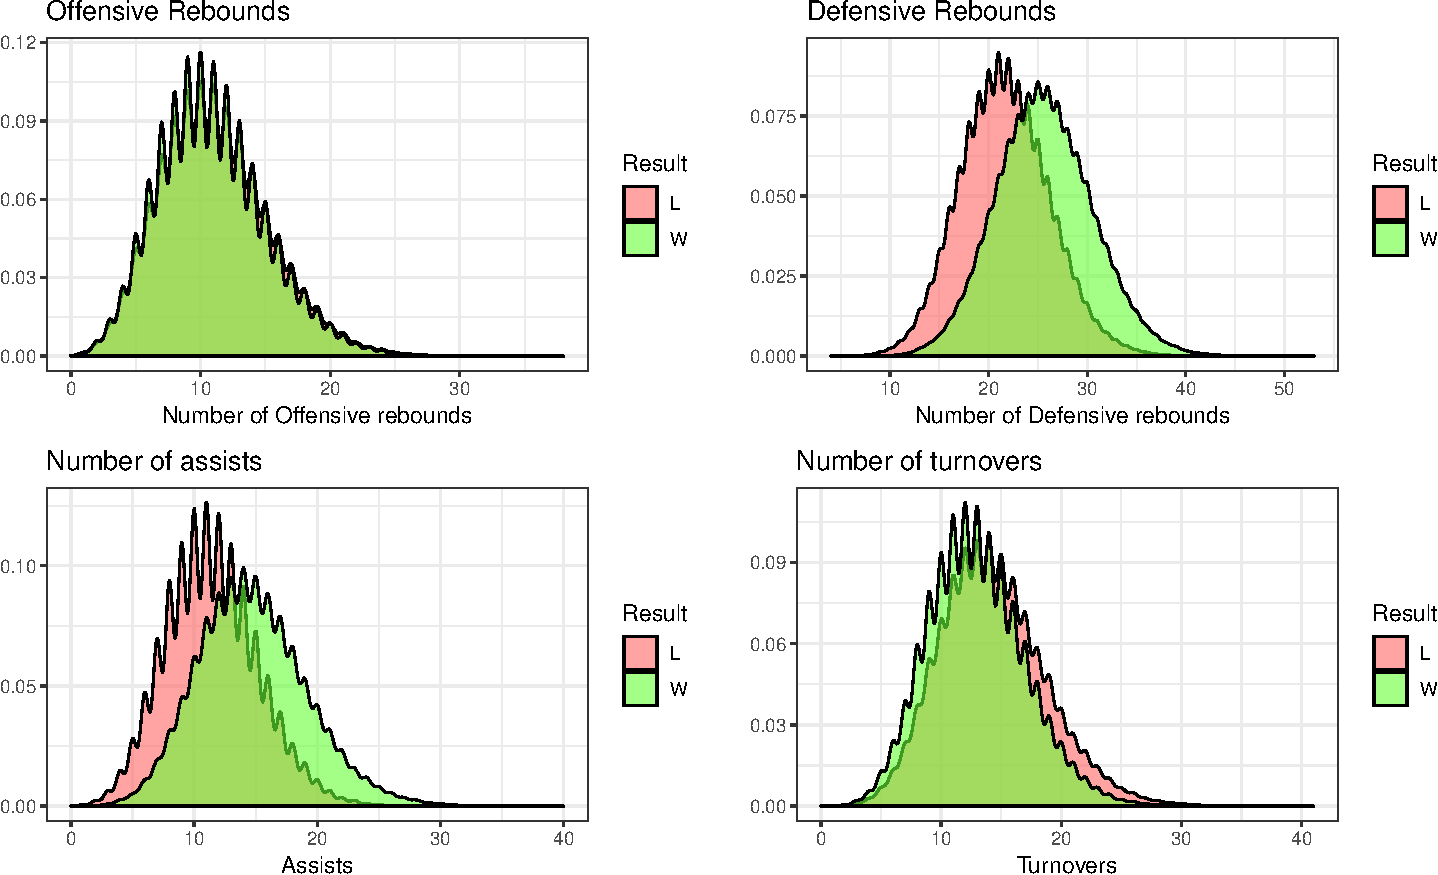
\includegraphics{EDA_files/figure-latex/unnamed-chunk-6-1.pdf}

Unsurprisingly, we see that winning teams tend to have a higher mean (or
lower in the case of turnover) in pretty much every metric. The last few
plots are bit spikey due to the more discrete nature of the data.

We don't have final game statistics until we have the Result, so we
obviously can't use these statistics in this form to predict the winners
of tournament matchups. However, we can use regular season aggregate
statistics to predict the winner in tournament matchups. Let's take a
look at that next.

\subsection{Predictors of Tournament Success}\label{predictors}

One of the obvious predictors for how deep a team goes in the tournament
would be regular season wins. Let's see how regular season wins
correlate to tournament progress each year.

\begin{Shaded}
\begin{Highlighting}[]
\NormalTok{wins_s <-}\StringTok{ }\NormalTok{seas_results[, .(}\DataTypeTok{rsW =}\NormalTok{ .N), by =}\StringTok{ }\KeywordTok{c}\NormalTok{(}\StringTok{'WTeamID'}\NormalTok{, }\StringTok{'Season'}\NormalTok{)] }\CommentTok{#Wins of a team per season}

\NormalTok{wins_t <-}\StringTok{ }\NormalTok{tour_results[}\OperatorTok{!}\NormalTok{(DayNum }\OperatorTok\StringTok{ }\KeywordTok{c}\NormalTok{(}\DecValTok{134}\NormalTok{, }\DecValTok{135}\NormalTok{)), .(}\DataTypeTok{tW =}\NormalTok{ .N), by =}\StringTok{ }\KeywordTok{c}\NormalTok{(}\StringTok{'WTeamID'}\NormalTok{, }\StringTok{'Season'}\NormalTok{)]}

\CommentTok{#max(wins_t$tW)}

\NormalTok{wins_teams <-}\StringTok{ }\NormalTok{wins_s[wins_t][teams]}
\end{Highlighting}
\end{Shaded}

In nearly every year, tournament wins is positively correlated with
regular season wins. Of course, there are some exceptions - for example
in 2000, the relationship is slightly negative! Single-elimination
tournaments produce some variations as they leave little room for error.
Sometimes strong favorites don't get as far as expected.

The problem with using regular season wins is that in college
basketball, not every team plays the same number of games in a regular
season. Let's do something similar to see if average scores during
regular season are associated with better tournament progress.

\begin{Shaded}
\begin{Highlighting}[]
\NormalTok{wins <-}\StringTok{ }\NormalTok{seas_results[, .(}\DataTypeTok{n_games =}\NormalTok{ .N, }\DataTypeTok{sum_score =} \KeywordTok{sum}\NormalTok{(WScore)), by =}\StringTok{ }\KeywordTok{c}\NormalTok{(}\StringTok{'WTeamID'}\NormalTok{, }\StringTok{'Season'}\NormalTok{)]}

\NormalTok{losses <-}\StringTok{ }\NormalTok{seas_results[, .(}\DataTypeTok{n_games =}\NormalTok{ .N, }\DataTypeTok{sum_score =} \KeywordTok{sum}\NormalTok{(LScore)), by =}\StringTok{ }\KeywordTok{c}\NormalTok{(}\StringTok{'LTeamID'}\NormalTok{, }\StringTok{'Season'}\NormalTok{)]}

\NormalTok{all_games <-}\StringTok{ }\KeywordTok{rbindlist}\NormalTok{(}\KeywordTok{list}\NormalTok{(wins, losses))}

\NormalTok{all_games <-}\StringTok{ }\NormalTok{all_games[, .(}\DataTypeTok{rs_ppg =} \KeywordTok{sum}\NormalTok{(sum_score) }\OperatorTok{/}\StringTok{ }\KeywordTok{sum}\NormalTok{(n_games)), by =}\StringTok{ }\KeywordTok{c}\NormalTok{(}\StringTok{'WTeamID'}\NormalTok{, }\StringTok{'Season'}\NormalTok{)]}
\end{Highlighting}
\end{Shaded}

\begin{Shaded}
\begin{Highlighting}[]
\NormalTok{seeds[, .(Season, }\DataTypeTok{WTeamID =}\NormalTok{ TeamID, }\DataTypeTok{seed_num =} \KeywordTok{as.numeric}\NormalTok{(}\KeywordTok{substr}\NormalTok{(Seed, }\DecValTok{2}\NormalTok{, }\DecValTok{3}\NormalTok{)))}
\NormalTok{      ][wins_t, on =}\StringTok{ }\KeywordTok{c}\NormalTok{(}\StringTok{'Season'}\NormalTok{, }\StringTok{'WTeamID'}\NormalTok{)] }\OperatorTok
\StringTok{    }\KeywordTok{ggplot}\NormalTok{(}\KeywordTok{aes}\NormalTok{(}\DataTypeTok{x =}\NormalTok{ seed_num, }\DataTypeTok{y =}\NormalTok{ tW)) }\OperatorTok{+}\StringTok{ }
\StringTok{    }\KeywordTok{geom_jitter}\NormalTok{(}\DataTypeTok{width =} \FloatTok{0.2}\NormalTok{, }\DataTypeTok{height =} \FloatTok{0.2}\NormalTok{) }\OperatorTok{+}\StringTok{ }
\StringTok{    }\KeywordTok{geom_smooth}\NormalTok{(}\DataTypeTok{method =} \StringTok{'lm'}\NormalTok{) }\OperatorTok{+}\StringTok{ }
\StringTok{    }\KeywordTok{labs}\NormalTok{(}
        \DataTypeTok{x =} \StringTok{'Seed'}\NormalTok{, }
        \DataTypeTok{y =} \StringTok{'Tournament Wins'}\NormalTok{, }
        \DataTypeTok{title =} \StringTok{'Tournament Wins by Seed'}\NormalTok{)}
\end{Highlighting}
\end{Shaded}

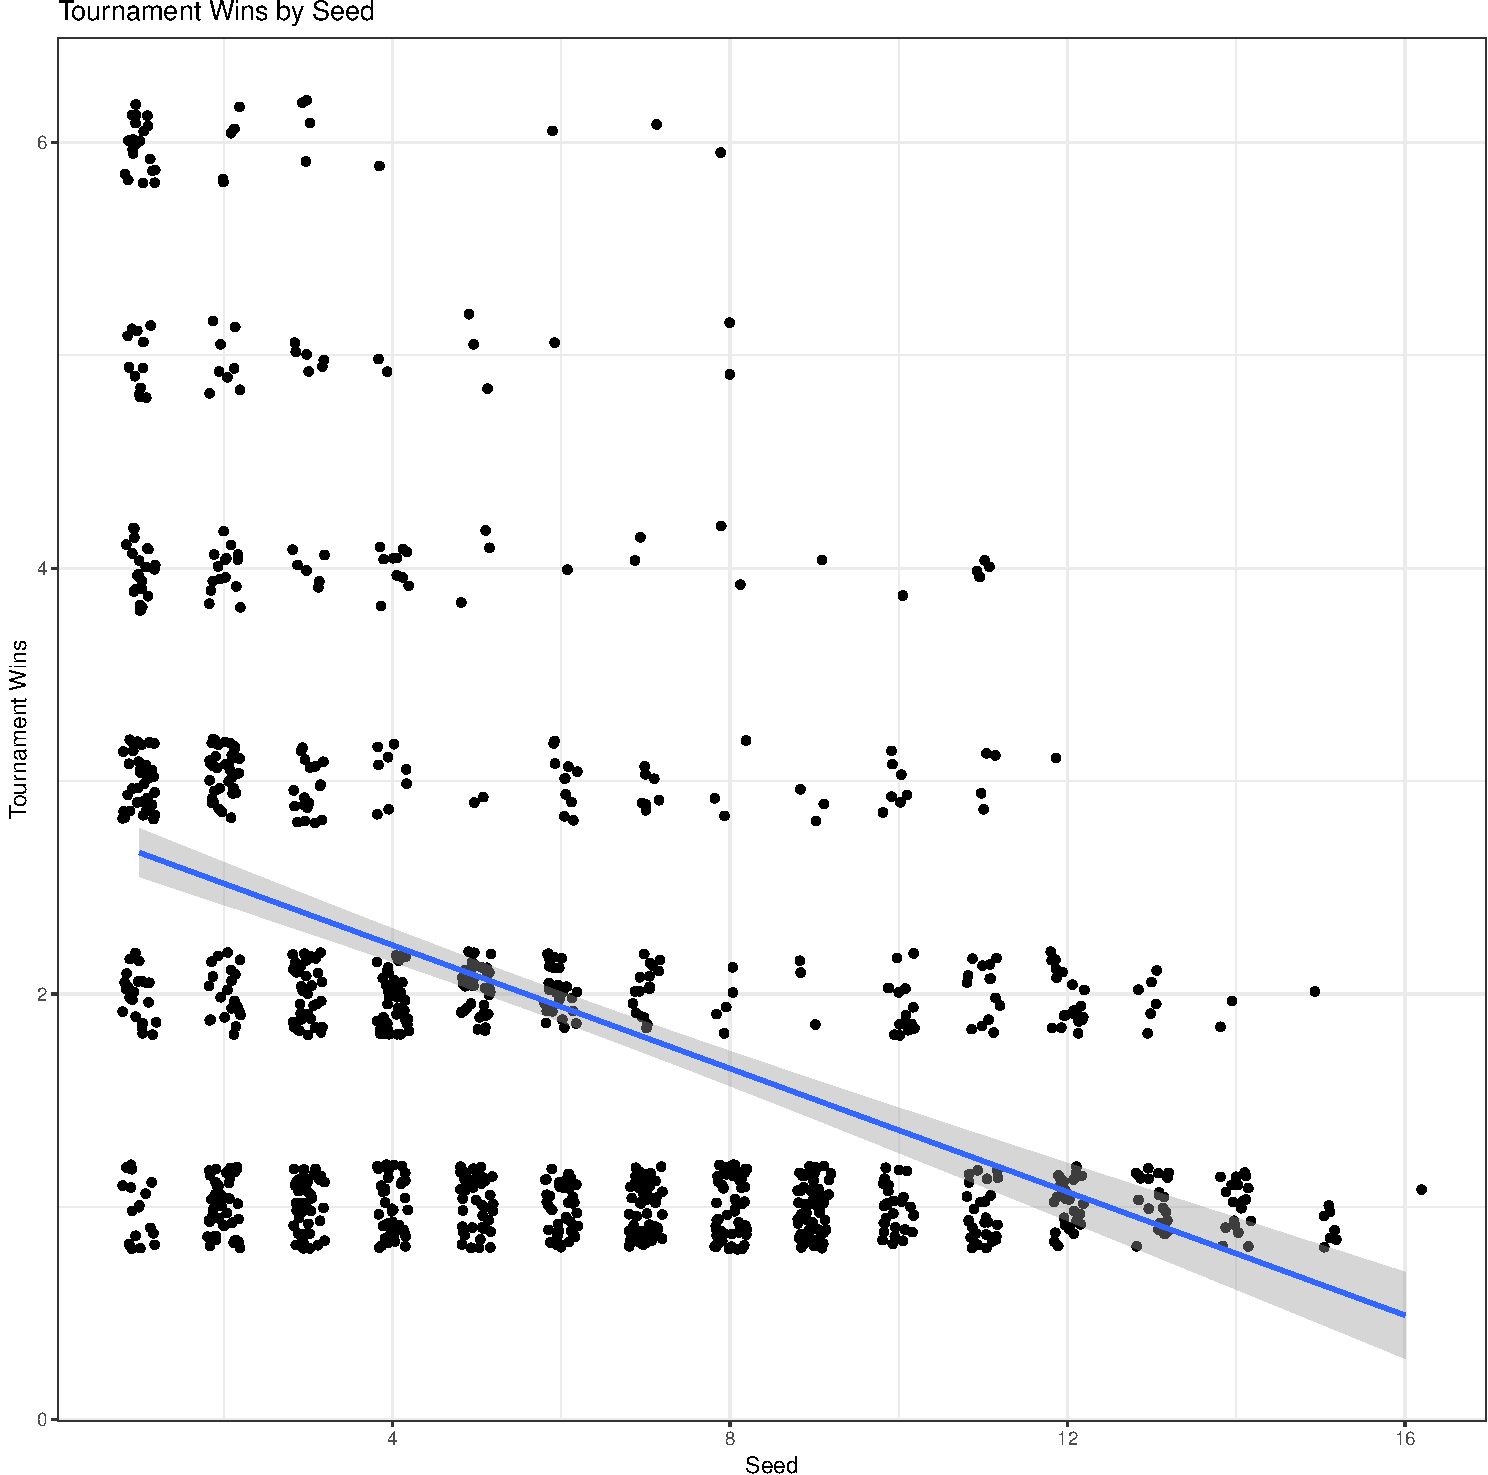
\includegraphics{EDA_files/figure-latex/unnamed-chunk-9-1.pdf}

I've introduced some jiter to this plot to avoid overplotting. It
exhibits a strong negative relationship between seed and tournament
progress - the lower a team's seed, the deeper they go into the
tournament (as measured by tournament wins). We see that a 16 seed has
never made it past the first round of the tournament. From the plot we
can also determine that the lowest seed to ever win the tournament was a
number 8. A vast majority of teams that have won the tournament since
1985 have been number 1 seeds.

We may also wonder how likely it is that a better-seeded (i.e.~lower
number) team will win any particular tournament matchup. Let's look at
the percentage of times the better-seeded team won by season.

\begin{Shaded}
\begin{Highlighting}[]
\NormalTok{tour_results_seeds <-}\StringTok{ }\NormalTok{seeds[, .(Season, }\DataTypeTok{WTeamID =}\NormalTok{ TeamID, }\DataTypeTok{winner_seed =} \KeywordTok{as.numeric}\NormalTok{(}\KeywordTok{substr}\NormalTok{(Seed, }\DecValTok{2}\NormalTok{, }\DecValTok{3}\NormalTok{)))}
\NormalTok{                            ][tour_results, on =}\StringTok{ }\KeywordTok{c}\NormalTok{(}\StringTok{'Season'}\NormalTok{, }\StringTok{'WTeamID'}\NormalTok{)}
\NormalTok{                              ][seeds[, .(Season, }\DataTypeTok{LTeamID =}\NormalTok{ TeamID, }\DataTypeTok{loser_seed =} \KeywordTok{as.numeric}\NormalTok{(}\KeywordTok{substr}\NormalTok{(Seed, }\DecValTok{2}\NormalTok{, }\DecValTok{3}\NormalTok{)))}
\NormalTok{                                      ], on =}\StringTok{ }\KeywordTok{c}\NormalTok{(}\StringTok{'Season'}\NormalTok{, }\StringTok{'LTeamID'}\NormalTok{)]}



\NormalTok{tour_results_seeds[Season }\OperatorTok{!=}\StringTok{ }\DecValTok{2018}\NormalTok{, .(Season, }\DataTypeTok{low_seed_win =} \KeywordTok{ifelse}\NormalTok{(winner_seed }\OperatorTok{<}\StringTok{ }\NormalTok{loser_seed, }\DecValTok{1}\NormalTok{, }\DecValTok{0}\NormalTok{))}
\NormalTok{                   ][, }\KeywordTok{sum}\NormalTok{(low_seed_win, }\DataTypeTok{na.rm =} \OtherTok{TRUE}\NormalTok{) }\OperatorTok{/}\StringTok{ }\NormalTok{.N, by =}\StringTok{ }\NormalTok{Season] }\OperatorTok
\StringTok{    }\KeywordTok{ggplot}\NormalTok{(}\KeywordTok{aes}\NormalTok{(}\DataTypeTok{x =} \KeywordTok{reorder}\NormalTok{(Season, }\OperatorTok{-}\NormalTok{V1), }\DataTypeTok{y =}\NormalTok{ V1)) }\OperatorTok{+}\StringTok{ }
\StringTok{    }\KeywordTok{geom_point}\NormalTok{(}\DataTypeTok{color =} \StringTok{'darkblue'}\NormalTok{, }\DataTypeTok{size =} \DecValTok{2}\NormalTok{) }\OperatorTok{+}\StringTok{ }
\StringTok{    }\KeywordTok{labs}\NormalTok{(}
        \DataTypeTok{x =} \StringTok{''}\NormalTok{, }
        \DataTypeTok{y =} \StringTok{'% of games in which better-seeded team won'}\NormalTok{, }
        \DataTypeTok{title =} \StringTok{'Better-seed winning percentage by year'}\NormalTok{) }\OperatorTok{+}\StringTok{ }
\StringTok{    }\KeywordTok{theme}\NormalTok{(}\DataTypeTok{axis.text.x =} \KeywordTok{element_text}\NormalTok{(}\DataTypeTok{angle =} \DecValTok{90}\NormalTok{, }\DataTypeTok{hjust =} \DecValTok{1}\NormalTok{))}
\end{Highlighting}
\end{Shaded}

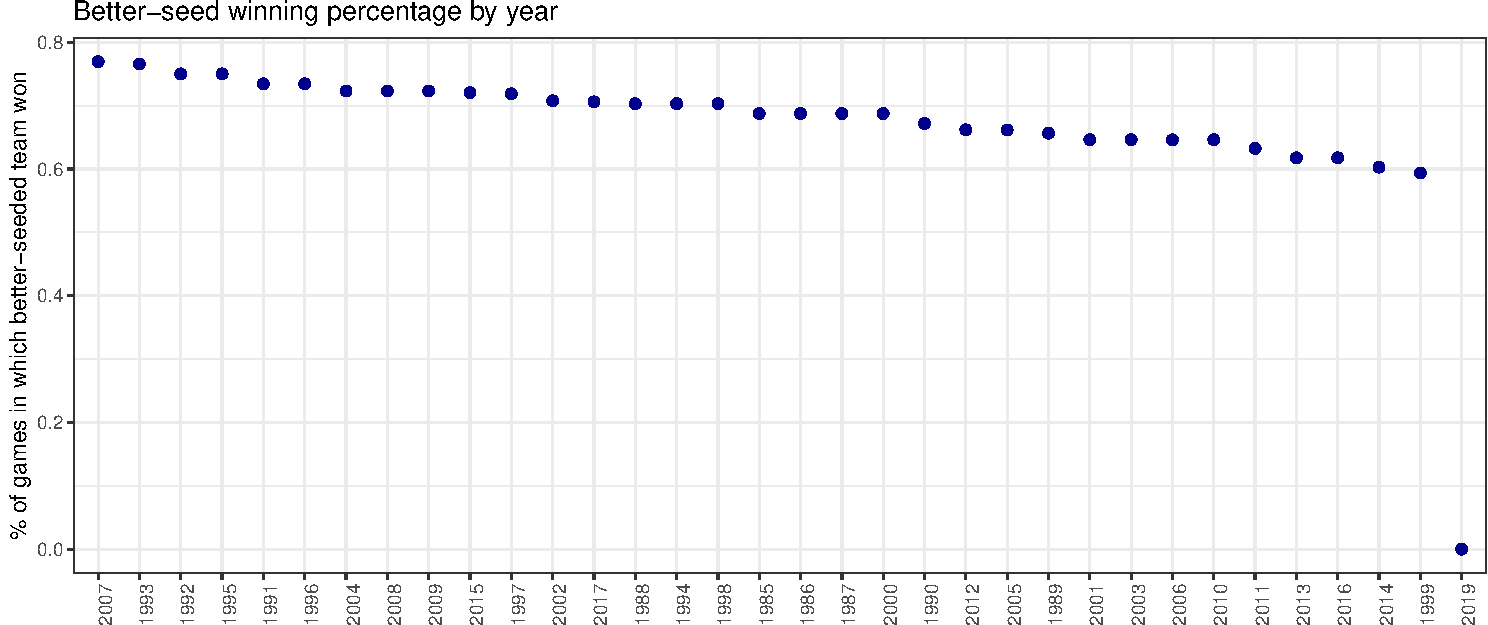
\includegraphics{EDA_files/figure-latex/unnamed-chunk-10-1.pdf}

When examining these data by season, we see that the better-seeded team
won games at a rate that varies between 0.79 in the 2007 tournament to
approximately 0.59 in the 1999 tournament.

Now let's examine the relationship between a team's regular season win
margin and its tournament performance.

\begin{Shaded}
\begin{Highlighting}[]
\NormalTok{seas_results[, .(}\DataTypeTok{avg_win_marg =} \KeywordTok{mean}\NormalTok{(WScore }\OperatorTok{-}\StringTok{ }\NormalTok{LScore)), by =}\StringTok{ }\KeywordTok{c}\NormalTok{(}\StringTok{'WTeamID'}\NormalTok{, }\StringTok{'Season'}\NormalTok{)}
\NormalTok{             ][wins_t, on =}\StringTok{ }\KeywordTok{c}\NormalTok{(}\StringTok{'WTeamID'}\NormalTok{, }\StringTok{'Season'}\NormalTok{)] }\OperatorTok
\StringTok{    }\KeywordTok{ggplot}\NormalTok{(}\KeywordTok{aes}\NormalTok{(}\DataTypeTok{x =}\NormalTok{ avg_win_marg, }\DataTypeTok{y =}\NormalTok{ tW)) }\OperatorTok{+}\StringTok{ }
\StringTok{    }\KeywordTok{geom_point}\NormalTok{() }\OperatorTok{+}\StringTok{ }
\StringTok{    }\KeywordTok{geom_smooth}\NormalTok{(}\DataTypeTok{method =} \StringTok{'lm'}\NormalTok{) }\OperatorTok{+}
\StringTok{    }\KeywordTok{labs}\NormalTok{(}
        \DataTypeTok{x =} \StringTok{'Average regular season win margin'}\NormalTok{, }
        \DataTypeTok{y =} \StringTok{'Tournament wins'}\NormalTok{, }
        \DataTypeTok{title =} \StringTok{'Tournament Wins by Regular Season Win Margin'}\NormalTok{) }\OperatorTok{+}\StringTok{ }
\StringTok{    }\KeywordTok{facet_wrap}\NormalTok{(}\OperatorTok{~}\NormalTok{Season) }
\end{Highlighting}
\end{Shaded}

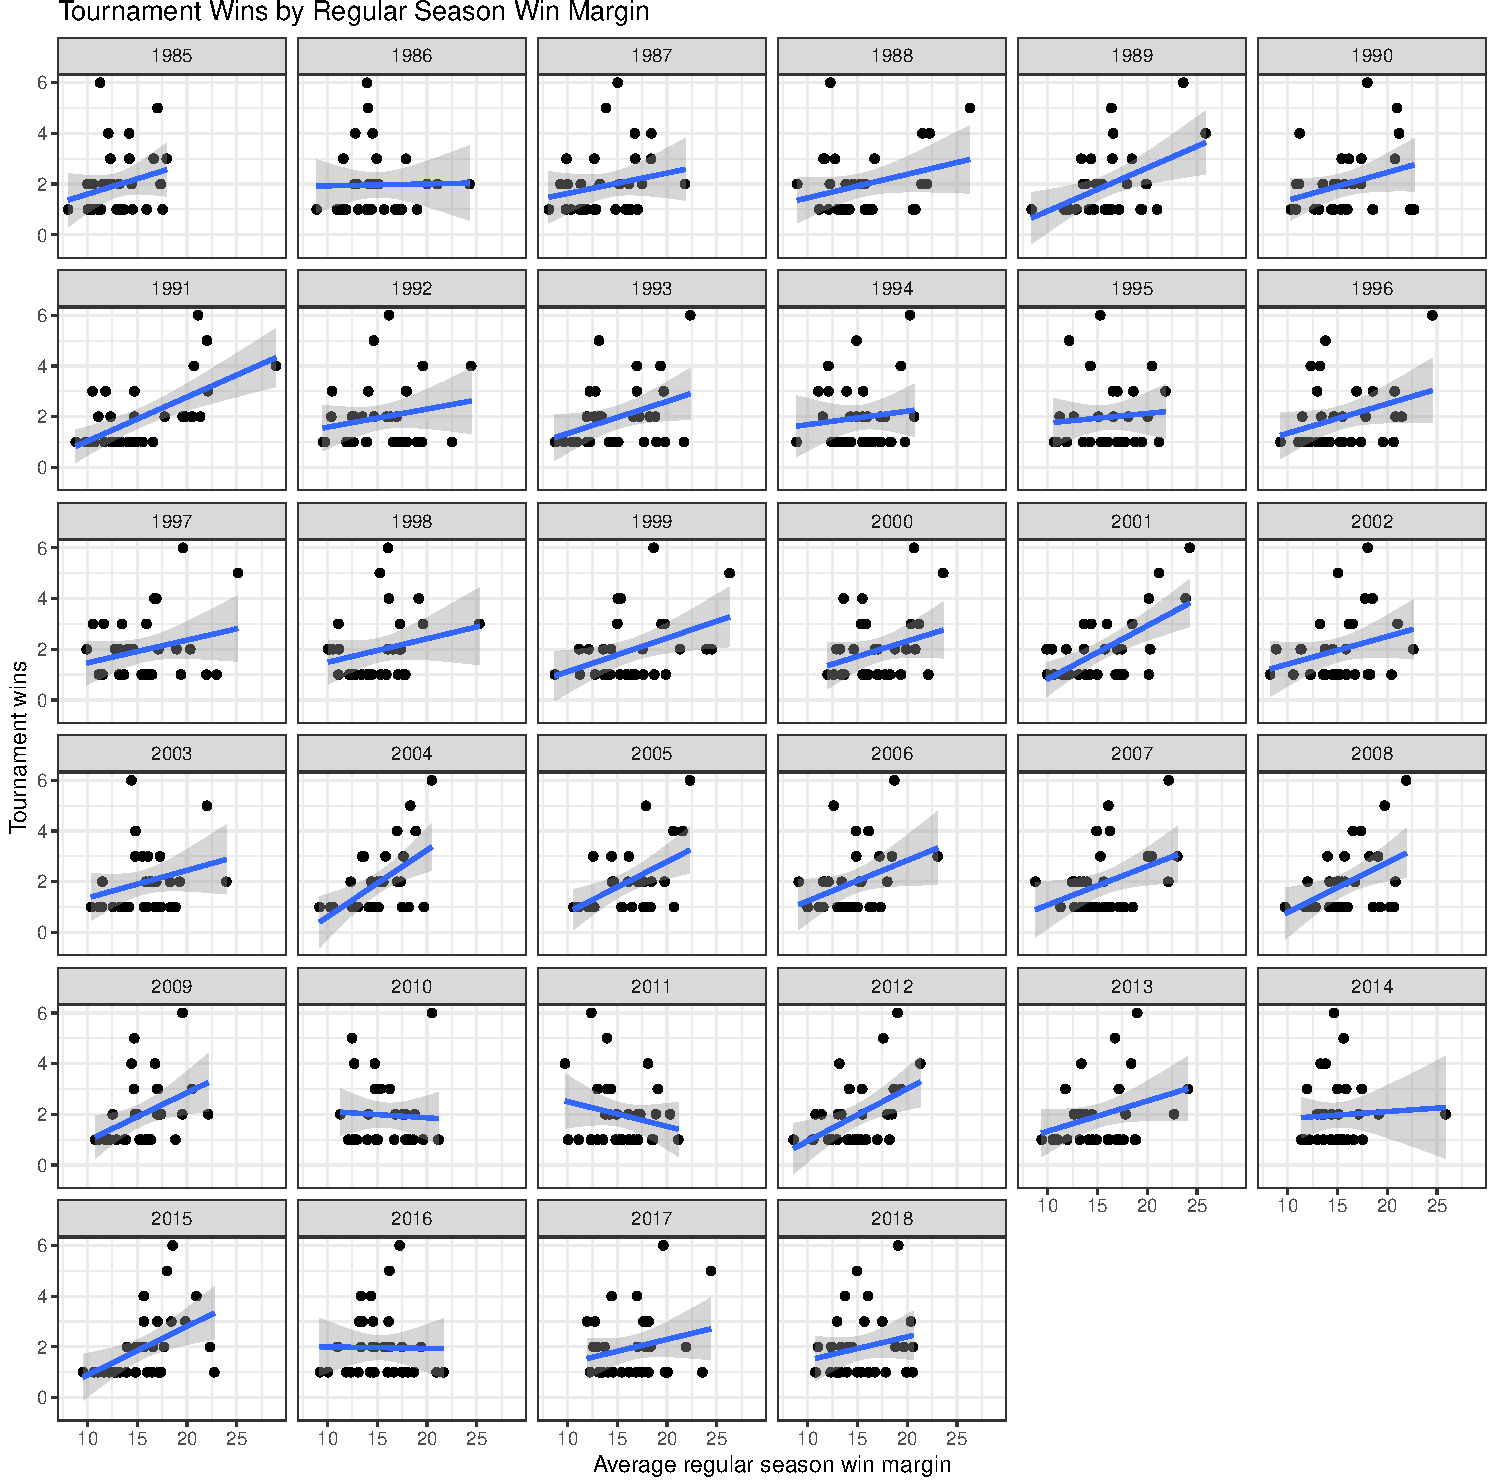
\includegraphics{EDA_files/figure-latex/unnamed-chunk-11-1.pdf}

Now let's move beyond the basic stats and use some of the box score data
as well. To start, let's create a standardized data frame in wide format
with all of the teams regular season stats. We'll create some additional
statistics such as various shooting percentages, rebounds per game,
steals per game, etc. Because of the format of the data, we first need
to get the stats for the games winning teams and losing teams
seperately. Then we will bind these row-wise and group by Season and
TeamID to calculate the stats.

\begin{Shaded}
\begin{Highlighting}[]
\CommentTok{#stats_season -> average}
\NormalTok{stats_season <-}\StringTok{ }\NormalTok{stats_all[, .(}
    \DataTypeTok{FGP =} \KeywordTok{sum}\NormalTok{(FGM) }\OperatorTok{/}\StringTok{ }\KeywordTok{sum}\NormalTok{(FGA),}
    \DataTypeTok{FGP3 =} \KeywordTok{sum}\NormalTok{(FGM3) }\OperatorTok{/}\StringTok{ }\KeywordTok{sum}\NormalTok{(FGA3),}
    \DataTypeTok{FTP =} \KeywordTok{sum}\NormalTok{(FTM) }\OperatorTok{/}\StringTok{ }\KeywordTok{sum}\NormalTok{(FTA),}
    \DataTypeTok{ORPG =} \KeywordTok{mean}\NormalTok{(OR),}
    \DataTypeTok{DRPG =} \KeywordTok{mean}\NormalTok{(DR),}
    \DataTypeTok{ASPG =} \KeywordTok{mean}\NormalTok{(AST),}
    \DataTypeTok{TOPG =} \KeywordTok{mean}\NormalTok{(TO),}
    \DataTypeTok{STPG =} \KeywordTok{mean}\NormalTok{(STL),}
    \CommentTok{#MFTAR = mean(FTAR),}
    \CommentTok{#BLPG = mean(BLK),}
    \CommentTok{#PFPG = mean(PF),}
    \DataTypeTok{MeFG =} \KeywordTok{mean}\NormalTok{(eFG),}
    \DataTypeTok{MNetRTG =} \KeywordTok{mean}\NormalTok{(NetRTG),}
    \CommentTok{#MORP = mean(ORP),}
    \DataTypeTok{MPIE =} \KeywordTok{mean}\NormalTok{(PIE),}
    \DataTypeTok{MPOS =} \KeywordTok{mean}\NormalTok{(POS),}
    \DataTypeTok{EFG =}\NormalTok{ (}\KeywordTok{mean}\NormalTok{(FGM)}\OperatorTok{+}\FloatTok{0.5}\OperatorTok{*}\KeywordTok{mean}\NormalTok{(FGM3))}\OperatorTok{/}\KeywordTok{mean}\NormalTok{(FGA))}
    
\NormalTok{    , by =}\StringTok{ }\KeywordTok{c}\NormalTok{(}\StringTok{'TeamID'}\NormalTok{, }\StringTok{'Season'}\NormalTok{)]}
\NormalTok{seas_elos <-}\StringTok{ }\KeywordTok{fread}\NormalTok{(}\KeywordTok{paste}\NormalTok{(dir,}\StringTok{'season_elos.csv'}\NormalTok{,}\DataTypeTok{sep=}\StringTok{''}\NormalTok{))}
\NormalTok{seas_elo_duke <-seas_elos[seas_elos}\OperatorTok{$}\NormalTok{team_id}\OperatorTok{==}\DecValTok{1181}\NormalTok{]}
\NormalTok{seas_elo_virginia <-seas_elos[seas_elos}\OperatorTok{$}\NormalTok{team_id}\OperatorTok{==}\DecValTok{1438}\NormalTok{]}
\NormalTok{seas_elo_virginia[seas_elo_virginia}\OperatorTok{==}\DecValTok{1438}\NormalTok{] <-}\StringTok{ "Virginia"}
\NormalTok{seas_elo_texas <-seas_elos[seas_elos}\OperatorTok{$}\NormalTok{team_id}\OperatorTok{==}\DecValTok{1403}\NormalTok{]}
\NormalTok{seas_elo_texas[seas_elo_texas}\OperatorTok{==}\DecValTok{1403}\NormalTok{] <-}\StringTok{ "Texas Tech"}
\NormalTok{seas_elo_michigan <-seas_elos[seas_elos}\OperatorTok{$}\NormalTok{team_id}\OperatorTok{==}\DecValTok{1277}\NormalTok{]}
\NormalTok{seas_elo_michigan[seas_elo_michigan}\OperatorTok{==}\DecValTok{1277}\NormalTok{] <-}\StringTok{ "Michigan St"}
\NormalTok{seas_elo_auburn <-seas_elos[seas_elos}\OperatorTok{$}\NormalTok{team_id}\OperatorTok{==}\DecValTok{1120}\NormalTok{]}
\NormalTok{seas_elo_auburn[seas_elo_auburn}\OperatorTok{==}\DecValTok{1120}\NormalTok{] <-}\StringTok{ "Auburn"}

\NormalTok{elos_plot <-}\StringTok{ }\KeywordTok{rbind}\NormalTok{(seas_elo_virginia,seas_elo_texas,seas_elo_michigan,seas_elo_auburn)}
\NormalTok{elos_plot}\OperatorTok{$}\NormalTok{team_id <-}\StringTok{ }\KeywordTok{as.factor}\NormalTok{(elos_plot}\OperatorTok{$}\NormalTok{team_id)}


\KeywordTok{ggplot}\NormalTok{(}\DataTypeTok{data=}\NormalTok{elos_plot, }\KeywordTok{aes}\NormalTok{(}\DataTypeTok{x=}\NormalTok{season, }\DataTypeTok{y=}\NormalTok{season_elo, }\DataTypeTok{group=}\NormalTok{team_id)) }\OperatorTok{+}
\StringTok{  }\CommentTok{#geom_point(aes(x=seas_elos$season, y=seas_elos$season_elo), size = 3) +}
\StringTok{  }\KeywordTok{geom_line}\NormalTok{(}\KeywordTok{aes}\NormalTok{(}\DataTypeTok{color=}\NormalTok{team_id))}\OperatorTok{+}
\StringTok{  }\CommentTok{#scale_color_brewer(palette="Paired")+}
\StringTok{  }\KeywordTok{theme_minimal}\NormalTok{() }\OperatorTok{+}
\StringTok{  }\KeywordTok{scale_fill_discrete}\NormalTok{(}\DataTypeTok{name =} \StringTok{"Teams"}\NormalTok{) }\OperatorTok{+}
\StringTok{  }\KeywordTok{labs}\NormalTok{(}\DataTypeTok{x =} \StringTok{"Year"}\NormalTok{) }\OperatorTok{+}\StringTok{ }\KeywordTok{labs}\NormalTok{(}\DataTypeTok{y =} \StringTok{"Elo Points"}\NormalTok{)}\OperatorTok{+}
\StringTok{  }\KeywordTok{labs}\NormalTok{(}\DataTypeTok{color=}\StringTok{"Colours"}\NormalTok{)}
\end{Highlighting}
\end{Shaded}

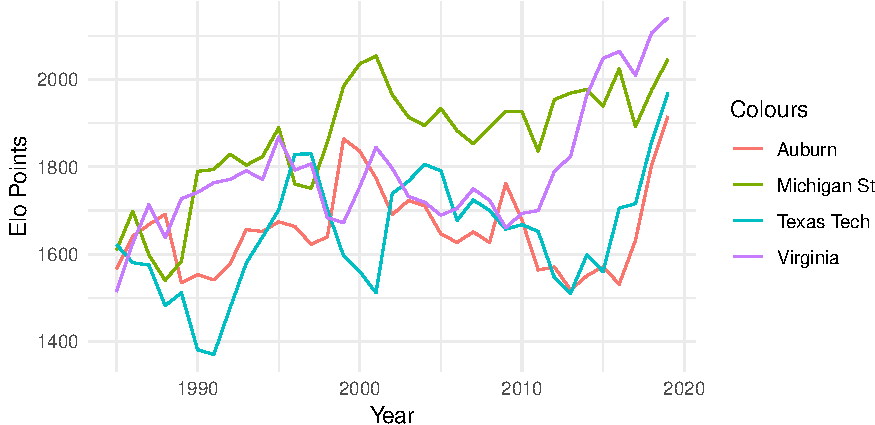
\includegraphics{EDA_files/figure-latex/unnamed-chunk-12-1.pdf}

\begin{Shaded}
\begin{Highlighting}[]
\KeywordTok{ggplot}\NormalTok{(}\DataTypeTok{data=}\NormalTok{seas_elo_virginia, }\KeywordTok{aes}\NormalTok{(}\DataTypeTok{x=}\NormalTok{seas_elo_virginia}\OperatorTok{$}\NormalTok{season, }\DataTypeTok{y=}\NormalTok{seas_elo_virginia}\OperatorTok{$}\NormalTok{season_elo)) }\OperatorTok{+}
\StringTok{  }\CommentTok{#geom_point(aes(x=seas_elos$season, y=seas_elos$season_elo), size = 3) +}
\StringTok{  }\KeywordTok{geom_line}\NormalTok{(}\DataTypeTok{color=}\StringTok{"blue"}\NormalTok{)}\OperatorTok{+}
\StringTok{  }\KeywordTok{scale_color_brewer}\NormalTok{(}\DataTypeTok{palette=}\StringTok{"Paired"}\NormalTok{)}\OperatorTok{+}
\StringTok{  }\KeywordTok{theme_minimal}\NormalTok{() }\OperatorTok{+}
\StringTok{  }\KeywordTok{labs}\NormalTok{(}\DataTypeTok{x =} \StringTok{"Year"}\NormalTok{) }\OperatorTok{+}\StringTok{ }\KeywordTok{labs}\NormalTok{(}\DataTypeTok{y =} \StringTok{"Elo Points"}\NormalTok{)}\OperatorTok{+}
\StringTok{  }\KeywordTok{labs}\NormalTok{(}\DataTypeTok{color=}\StringTok{"Colours"}\NormalTok{)}
\end{Highlighting}
\end{Shaded}

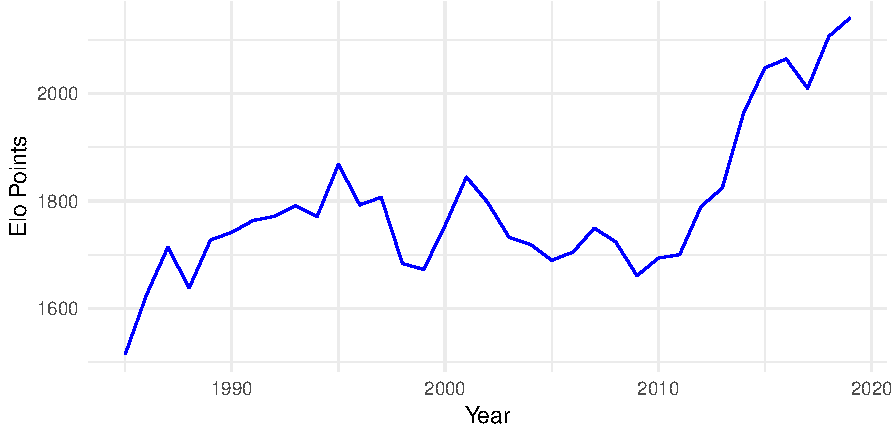
\includegraphics{EDA_files/figure-latex/unnamed-chunk-12-2.pdf}

\begin{Shaded}
\begin{Highlighting}[]
\NormalTok{seas_elos <-}\StringTok{ }\NormalTok{seas_elos[seas_elos}\OperatorTok{$}\NormalTok{season}\OperatorTok{>=}\DecValTok{2003}\NormalTok{,]}

\KeywordTok{colnames}\NormalTok{(seas_elos) <-}\KeywordTok{c}\NormalTok{(}\StringTok{"TeamID"}\NormalTok{,}\StringTok{"Season"}\NormalTok{,}\StringTok{"Season_elo"}\NormalTok{)}
\NormalTok{stats_season <-}\StringTok{ }\KeywordTok{merge}\NormalTok{(}\DataTypeTok{x =}\NormalTok{ stats_season, }\DataTypeTok{y =}\NormalTok{ seas_elos, }\DataTypeTok{by=}\KeywordTok{c}\NormalTok{(}\StringTok{"TeamID"}\NormalTok{,}\StringTok{"Season"}\NormalTok{), }\DataTypeTok{all =} \OtherTok{FALSE}\NormalTok{)}
\NormalTok{wins_t_}\DecValTok{2003}\NormalTok{ <-}\StringTok{ }\NormalTok{wins_t[wins_t}\OperatorTok{$}\NormalTok{Season}\OperatorTok{>=}\DecValTok{2003}\NormalTok{,]}
\KeywordTok{colnames}\NormalTok{(wins_t_}\DecValTok{2003}\NormalTok{) <-}\KeywordTok{c}\NormalTok{(}\StringTok{"TeamID"}\NormalTok{,}\StringTok{"Season"}\NormalTok{,}\StringTok{"Days_Tournament"}\NormalTok{)}
\NormalTok{stats_season <-}\StringTok{ }\KeywordTok{merge}\NormalTok{(}\DataTypeTok{x =}\NormalTok{ stats_season, }\DataTypeTok{y =}\NormalTok{ wins_t_}\DecValTok{2003}\NormalTok{, }\DataTypeTok{by=}\KeywordTok{c}\NormalTok{(}\StringTok{"TeamID"}\NormalTok{,}\StringTok{"Season"}\NormalTok{), }\DataTypeTok{all =} \OtherTok{FALSE}\NormalTok{)}
\NormalTok{dseeds_tournament <-}\StringTok{ }\KeywordTok{fread}\NormalTok{(}\KeywordTok{paste}\NormalTok{(dir,}\StringTok{'NCAATourneySeeds.csv'}\NormalTok{,}\DataTypeTok{sep=}\StringTok{''}\NormalTok{))}
\NormalTok{dseeds_tournament <-}\StringTok{ }\NormalTok{dseeds_tournament }\OperatorTok\StringTok{ }
\StringTok{  }\KeywordTok{mutate}\NormalTok{(}\DataTypeTok{ranking =} \KeywordTok{as.factor}\NormalTok{((}\KeywordTok{str_replace}\NormalTok{(Seed, }\StringTok{"[A-Z]"}\NormalTok{,}\StringTok{""}\NormalTok{))), }
         \DataTypeTok{rank_num =} \KeywordTok{as.numeric}\NormalTok{(}\KeywordTok{str_replace}\NormalTok{(ranking, }\StringTok{".[a-z]"}\NormalTok{,}\StringTok{""}\NormalTok{)))}
\NormalTok{dseeds_tournament <-}\StringTok{ }\NormalTok{dseeds_tournament[ , }\OperatorTok{-}\KeywordTok{which}\NormalTok{(}\KeywordTok{names}\NormalTok{(dseeds_tournament) }\OperatorTok\StringTok{ }\KeywordTok{c}\NormalTok{(}\StringTok{"Seed"}\NormalTok{,}\StringTok{"ranking"}\NormalTok{))]}
\CommentTok{#names(dseeds_tournament) <- tolower(names(dseeds_tournament))}
\NormalTok{stats_season <-}\StringTok{ }\KeywordTok{merge}\NormalTok{(}\DataTypeTok{x =}\NormalTok{ stats_season, }\DataTypeTok{y =}\NormalTok{ dseeds_tournament, }\DataTypeTok{by=}\KeywordTok{c}\NormalTok{(}\StringTok{"TeamID"}\NormalTok{,}\StringTok{"Season"}\NormalTok{), }\DataTypeTok{all =} \OtherTok{FALSE}\NormalTok{)}

\NormalTok{pca_crypto <-}\StringTok{ }\KeywordTok{princomp}\NormalTok{(}\OperatorTok{~}\NormalTok{Season_elo}\OperatorTok{+}\NormalTok{EFG}\OperatorTok{+}\NormalTok{MPOS}\OperatorTok{+}\NormalTok{Days_Tournament}\OperatorTok{+}\NormalTok{MPIE}\OperatorTok{+}\NormalTok{MNetRTG,}\DataTypeTok{cor=}\OtherTok{TRUE}\NormalTok{, }\DataTypeTok{data=}\NormalTok{stats_season)}
\NormalTok{pca_crypto <-}\StringTok{ }\KeywordTok{PCA}\NormalTok{(stats_season,}\DataTypeTok{scale.unit =} \OtherTok{TRUE}\NormalTok{,}\DataTypeTok{graph =} \OtherTok{FALSE}\NormalTok{)}
\KeywordTok{fviz_pca_var}\NormalTok{(pca_crypto, }\DataTypeTok{col.var =} \StringTok{"cos2"}\NormalTok{)}
\end{Highlighting}
\end{Shaded}

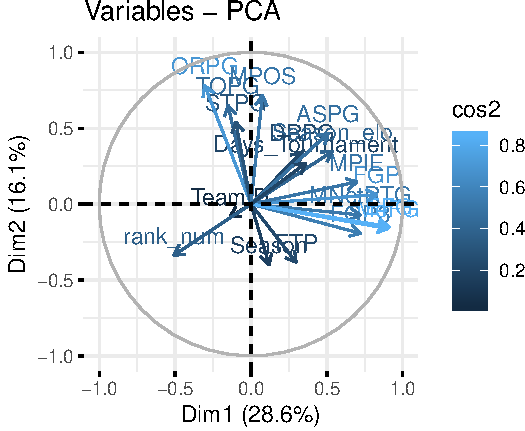
\includegraphics{EDA_files/figure-latex/unnamed-chunk-12-3.pdf}

\begin{Shaded}
\begin{Highlighting}[]
\NormalTok{M <-}\StringTok{ }\KeywordTok{cor}\NormalTok{(}\KeywordTok{scale}\NormalTok{(stats_season }\OperatorTok\StringTok{ }\KeywordTok{select}\NormalTok{ (}\DecValTok{3}\OperatorTok{:}\DecValTok{18}\NormalTok{)),}\DataTypeTok{method=}\StringTok{"pearson"}\NormalTok{)}
\KeywordTok{corrplot}\NormalTok{(M, }\DataTypeTok{method =} \StringTok{"circle"}\NormalTok{,}\DataTypeTok{type =} \StringTok{"upper"}\NormalTok{)}
\end{Highlighting}
\end{Shaded}

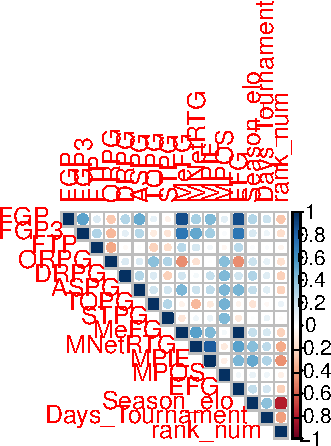
\includegraphics{EDA_files/figure-latex/unnamed-chunk-12-4.pdf}

\begin{Shaded}
\begin{Highlighting}[]
\CommentTok{#corrplot(stats_season, type = "upper", order = "hclust", }
         \CommentTok{#tl.col = "black")}
\end{Highlighting}
\end{Shaded}

Can we use a team's regular season game statistics to predict tournament
success. First let's look at field goal \% and free throw \% during the
regular season and see if these equate to tournament success. We'll
define success in the case as making the Final Four.

\begin{Shaded}
\begin{Highlighting}[]
\NormalTok{g1 <-}\StringTok{ }\NormalTok{stats_season[wins_t, on =}\StringTok{ }\KeywordTok{c}\NormalTok{(}\DataTypeTok{TeamID =} \StringTok{'WTeamID'}\NormalTok{, }\StringTok{'Season'}\NormalTok{), nomatch =}\StringTok{ }\DecValTok{0}
\NormalTok{              ][, final_four }\OperatorTok{:}\ErrorTok{=}\StringTok{ }\NormalTok{tW }\OperatorTok{>=}\StringTok{ }\DecValTok{4}\NormalTok{] }\OperatorTok
\StringTok{    }\KeywordTok{ggplot}\NormalTok{(}\KeywordTok{aes}\NormalTok{(}\DataTypeTok{x =}\NormalTok{ FGP, }\DataTypeTok{y =}\NormalTok{ FTP, }\DataTypeTok{color =}\NormalTok{ final_four)) }\OperatorTok{+}\StringTok{ }
\StringTok{    }\KeywordTok{geom_point}\NormalTok{(}\DataTypeTok{alpha =} \FloatTok{0.6}\NormalTok{) }\OperatorTok{+}
\StringTok{    }\KeywordTok{labs}\NormalTok{(}
        \DataTypeTok{x =} \StringTok{'Field goal %'}\NormalTok{, }
        \DataTypeTok{y =} \StringTok{'Free throw %'}\NormalTok{, }
        \DataTypeTok{title =} \StringTok{'Regular Season Shooting Performance of Tournament Teams'}\NormalTok{) }\OperatorTok{+}
\StringTok{    }\KeywordTok{scale_color_manual}\NormalTok{(}\DataTypeTok{values =} \KeywordTok{c}\NormalTok{(}\StringTok{'darkgrey'}\NormalTok{, }\StringTok{'steelblue'}\NormalTok{))}

\KeywordTok{ggMarginal}\NormalTok{(g1, }\DataTypeTok{type =} \StringTok{'histogram'}\NormalTok{, }\DataTypeTok{fill =} \StringTok{'steelblue'}\NormalTok{)}
\end{Highlighting}
\end{Shaded}

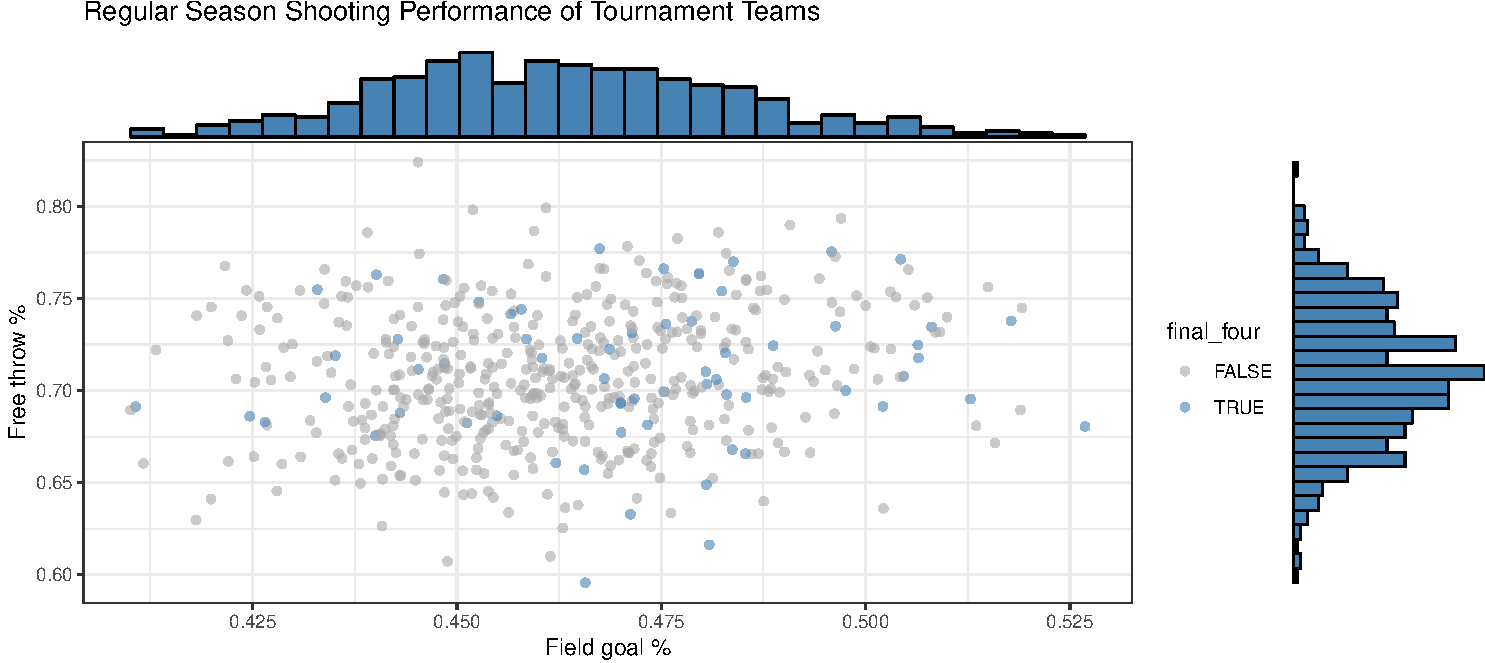
\includegraphics{EDA_files/figure-latex/unnamed-chunk-13-1.pdf}

We see that the distribution of field goal \% appears to have a peak
around 0.45. The distribution of free throw percentage peaks near 72\%.
Interestingly in terms of shooting \%, there does not seem to be much of
a difference between teams that make the Final Four and the rest of the
tournament field in terms of their regular season performance; however
it is hard to tell from this plot type. To double-check, let's plot the
densities of these two statistics for Final Four teams and the rest of
the field.

\begin{Shaded}
\begin{Highlighting}[]
\NormalTok{g1 <-}\StringTok{ }\NormalTok{stats_season[wins_t, on =}\StringTok{ }\KeywordTok{c}\NormalTok{(}\DataTypeTok{TeamID =} \StringTok{'WTeamID'}\NormalTok{, }\StringTok{'Season'}\NormalTok{), nomatch =}\StringTok{ }\DecValTok{0}
\NormalTok{              ][, final_four }\OperatorTok{:}\ErrorTok{=}\StringTok{ }\NormalTok{tW }\OperatorTok{>=}\StringTok{ }\DecValTok{4}\NormalTok{] }\OperatorTok
\StringTok{    }\KeywordTok{ggplot}\NormalTok{(}\KeywordTok{aes}\NormalTok{(}\DataTypeTok{x =}\NormalTok{ MPOS, }\DataTypeTok{fill =}\NormalTok{ final_four)) }\OperatorTok{+}\StringTok{ }
\StringTok{    }\KeywordTok{scale_fill_manual}\NormalTok{(}\DataTypeTok{values =} \KeywordTok{c}\NormalTok{(}\StringTok{'skyblue4'}\NormalTok{, }\StringTok{'skyblue3'}\NormalTok{)) }\OperatorTok{+}\StringTok{ }
\StringTok{    }\KeywordTok{geom_density}\NormalTok{(}\DataTypeTok{alpha =} \FloatTok{0.5}\NormalTok{) }\OperatorTok{+}\StringTok{ }
\StringTok{    }\KeywordTok{labs}\NormalTok{(}\DataTypeTok{x =} \StringTok{'Number of Possessions'}\NormalTok{, }\DataTypeTok{title =} \StringTok{'Regular Season Possessions'}\NormalTok{)}
\KeywordTok{grid.arrange}\NormalTok{(g1)}
\end{Highlighting}
\end{Shaded}

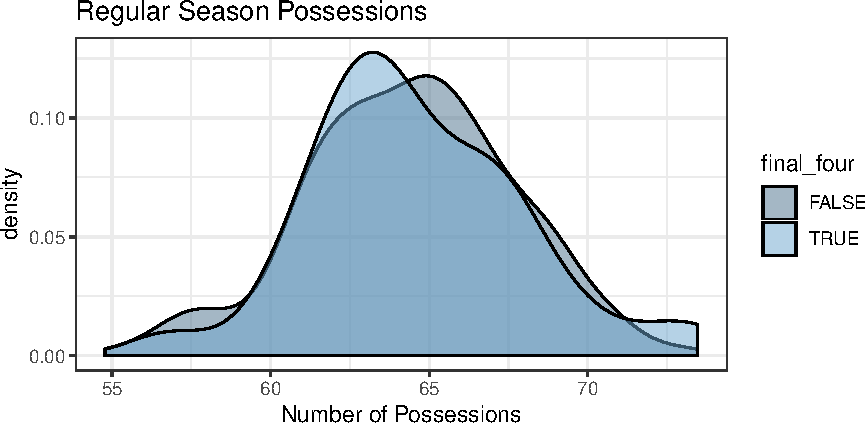
\includegraphics{EDA_files/figure-latex/unnamed-chunk-14-1.pdf}

\begin{Shaded}
\begin{Highlighting}[]
\NormalTok{g1 <-}\StringTok{ }\NormalTok{stats_season[wins_t, on =}\StringTok{ }\KeywordTok{c}\NormalTok{(}\DataTypeTok{TeamID =} \StringTok{'WTeamID'}\NormalTok{, }\StringTok{'Season'}\NormalTok{), nomatch =}\StringTok{ }\DecValTok{0}
\NormalTok{              ][, final_four }\OperatorTok{:}\ErrorTok{=}\StringTok{ }\NormalTok{tW }\OperatorTok{>=}\StringTok{ }\DecValTok{4}\NormalTok{] }\OperatorTok
\StringTok{    }\KeywordTok{ggplot}\NormalTok{(}\KeywordTok{aes}\NormalTok{(}\DataTypeTok{x =}\NormalTok{ MPIE, }\DataTypeTok{fill =}\NormalTok{ final_four)) }\OperatorTok{+}\StringTok{ }
\StringTok{    }\KeywordTok{scale_fill_manual}\NormalTok{(}\DataTypeTok{values =} \KeywordTok{c}\NormalTok{(}\StringTok{'skyblue4'}\NormalTok{, }\StringTok{'skyblue3'}\NormalTok{)) }\OperatorTok{+}\StringTok{ }
\StringTok{    }\KeywordTok{geom_density}\NormalTok{(}\DataTypeTok{alpha =} \FloatTok{0.5}\NormalTok{) }\OperatorTok{+}\StringTok{ }
\StringTok{    }\KeywordTok{labs}\NormalTok{(}\DataTypeTok{x =} \StringTok{'PIE'}\NormalTok{, }\DataTypeTok{title =} \StringTok{'Regular Season PIE'}\NormalTok{)}

\NormalTok{g2 <-}\StringTok{ }\NormalTok{stats_season[wins_t, on =}\StringTok{ }\KeywordTok{c}\NormalTok{(}\DataTypeTok{TeamID =} \StringTok{'WTeamID'}\NormalTok{, }\StringTok{'Season'}\NormalTok{), nomatch =}\StringTok{ }\DecValTok{0}
\NormalTok{              ][, final_four }\OperatorTok{:}\ErrorTok{=}\StringTok{ }\NormalTok{tW }\OperatorTok{>=}\StringTok{ }\DecValTok{4}\NormalTok{] }\OperatorTok
\StringTok{    }\KeywordTok{ggplot}\NormalTok{(}\KeywordTok{aes}\NormalTok{(}\DataTypeTok{x =}\NormalTok{ MNetRTG, }\DataTypeTok{fill =}\NormalTok{ final_four)) }\OperatorTok{+}\StringTok{ }
\StringTok{    }\KeywordTok{scale_fill_manual}\NormalTok{(}\DataTypeTok{values =} \KeywordTok{c}\NormalTok{(}\StringTok{'skyblue4'}\NormalTok{, }\StringTok{'skyblue3'}\NormalTok{)) }\OperatorTok{+}\StringTok{ }
\StringTok{    }\KeywordTok{geom_density}\NormalTok{(}\DataTypeTok{alpha =} \FloatTok{0.5}\NormalTok{) }\OperatorTok{+}\StringTok{ }
\StringTok{    }\KeywordTok{labs}\NormalTok{(}\DataTypeTok{x =} \StringTok{'Net Rating'}\NormalTok{, }\DataTypeTok{title =} \StringTok{'Regular Season Net Rating'}\NormalTok{)}

\NormalTok{g3 <-}\StringTok{ }\NormalTok{stats_season[wins_t, on =}\StringTok{ }\KeywordTok{c}\NormalTok{(}\DataTypeTok{TeamID =} \StringTok{'WTeamID'}\NormalTok{, }\StringTok{'Season'}\NormalTok{), nomatch =}\StringTok{ }\DecValTok{0}
\NormalTok{              ][, final_four }\OperatorTok{:}\ErrorTok{=}\StringTok{ }\NormalTok{tW }\OperatorTok{>=}\StringTok{ }\DecValTok{4}\NormalTok{] }\OperatorTok
\StringTok{    }\KeywordTok{ggplot}\NormalTok{(}\KeywordTok{aes}\NormalTok{(}\DataTypeTok{x =}\NormalTok{ Season_elo, }\DataTypeTok{fill =}\NormalTok{ final_four)) }\OperatorTok{+}\StringTok{ }
\StringTok{    }\KeywordTok{scale_fill_manual}\NormalTok{(}\DataTypeTok{values =} \KeywordTok{c}\NormalTok{(}\StringTok{'skyblue4'}\NormalTok{, }\StringTok{'skyblue3'}\NormalTok{)) }\OperatorTok{+}\StringTok{ }
\StringTok{    }\KeywordTok{geom_density}\NormalTok{(}\DataTypeTok{alpha =} \FloatTok{0.5}\NormalTok{) }\OperatorTok{+}\StringTok{ }
\StringTok{    }\KeywordTok{labs}\NormalTok{(}\DataTypeTok{x =} \StringTok{'Elo Rating'}\NormalTok{, }\DataTypeTok{title =} \StringTok{'Season ending Elo Rating'}\NormalTok{)}

\NormalTok{g4 <-}\StringTok{ }\NormalTok{stats_season[wins_t, on =}\StringTok{ }\KeywordTok{c}\NormalTok{(}\DataTypeTok{TeamID =} \StringTok{'WTeamID'}\NormalTok{, }\StringTok{'Season'}\NormalTok{), nomatch =}\StringTok{ }\DecValTok{0}
\NormalTok{              ][, final_four }\OperatorTok{:}\ErrorTok{=}\StringTok{ }\NormalTok{tW }\OperatorTok{>=}\StringTok{ }\DecValTok{4}\NormalTok{] }\OperatorTok
\StringTok{    }\KeywordTok{ggplot}\NormalTok{(}\KeywordTok{aes}\NormalTok{(}\DataTypeTok{x =}\NormalTok{ rank_num, }\DataTypeTok{fill =}\NormalTok{ final_four)) }\OperatorTok{+}\StringTok{ }
\StringTok{    }\KeywordTok{scale_fill_manual}\NormalTok{(}\DataTypeTok{values =} \KeywordTok{c}\NormalTok{(}\StringTok{'skyblue4'}\NormalTok{, }\StringTok{'skyblue3'}\NormalTok{)) }\OperatorTok{+}\StringTok{ }
\StringTok{    }\KeywordTok{geom_density}\NormalTok{(}\DataTypeTok{alpha =} \FloatTok{0.5}\NormalTok{) }\OperatorTok{+}\StringTok{ }
\StringTok{    }\KeywordTok{labs}\NormalTok{(}\DataTypeTok{x =} \StringTok{'Seeding position'}\NormalTok{, }\DataTypeTok{title =} \StringTok{'Ranking in seeding'}\NormalTok{)}


\KeywordTok{grid.arrange}\NormalTok{(g1, g2, g3, g4, }\DataTypeTok{ncol =} \DecValTok{2}\NormalTok{)}
\end{Highlighting}
\end{Shaded}

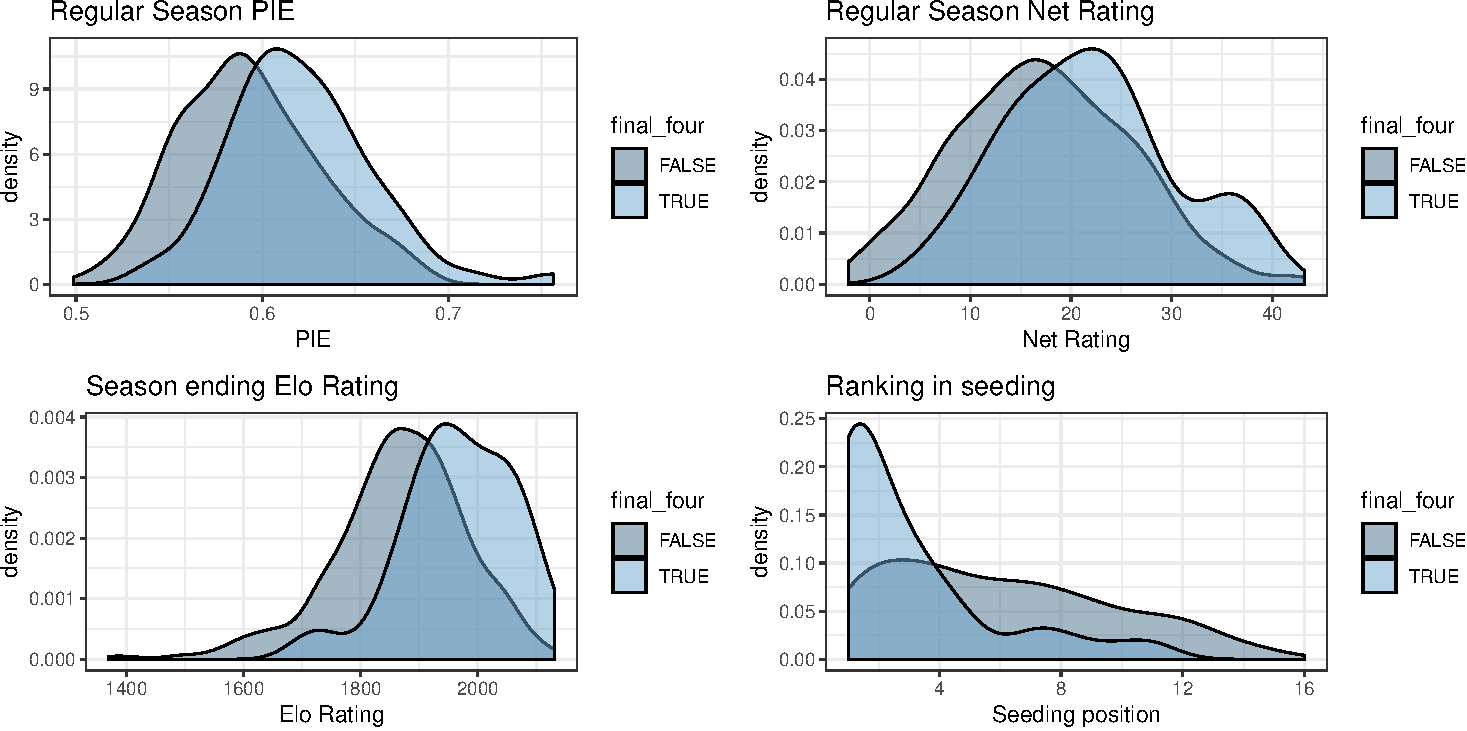
\includegraphics{EDA_files/figure-latex/unnamed-chunk-15-1.pdf}

\begin{Shaded}
\begin{Highlighting}[]
\NormalTok{g1 <-}\StringTok{ }\NormalTok{stats_season[wins_t, on =}\StringTok{ }\KeywordTok{c}\NormalTok{(}\DataTypeTok{TeamID =} \StringTok{'WTeamID'}\NormalTok{, }\StringTok{'Season'}\NormalTok{), nomatch =}\StringTok{ }\DecValTok{0}
\NormalTok{              ][, final_four }\OperatorTok{:}\ErrorTok{=}\StringTok{ }\NormalTok{tW }\OperatorTok{>=}\StringTok{ }\DecValTok{4}\NormalTok{] }\OperatorTok
\StringTok{    }\KeywordTok{ggplot}\NormalTok{(}\KeywordTok{aes}\NormalTok{(}\DataTypeTok{x =}\NormalTok{ FGP, }\DataTypeTok{fill =}\NormalTok{ final_four)) }\OperatorTok{+}\StringTok{ }
\StringTok{    }\KeywordTok{scale_fill_manual}\NormalTok{(}\DataTypeTok{values =} \KeywordTok{c}\NormalTok{(}\StringTok{'skyblue4'}\NormalTok{, }\StringTok{'skyblue3'}\NormalTok{)) }\OperatorTok{+}\StringTok{ }
\StringTok{    }\KeywordTok{geom_density}\NormalTok{(}\DataTypeTok{alpha =} \FloatTok{0.5}\NormalTok{) }\OperatorTok{+}\StringTok{ }
\StringTok{    }\KeywordTok{labs}\NormalTok{(}\DataTypeTok{x =} \StringTok{'PIE'}\NormalTok{, }\DataTypeTok{title =} \StringTok{'Regular Season PIE'}\NormalTok{)}

\NormalTok{g2 <-}\StringTok{ }\NormalTok{stats_season[wins_t, on =}\StringTok{ }\KeywordTok{c}\NormalTok{(}\DataTypeTok{TeamID =} \StringTok{'WTeamID'}\NormalTok{, }\StringTok{'Season'}\NormalTok{), nomatch =}\StringTok{ }\DecValTok{0}
\NormalTok{              ][, final_four }\OperatorTok{:}\ErrorTok{=}\StringTok{ }\NormalTok{tW }\OperatorTok{>=}\StringTok{ }\DecValTok{4}\NormalTok{] }\OperatorTok
\StringTok{    }\KeywordTok{ggplot}\NormalTok{(}\KeywordTok{aes}\NormalTok{(}\DataTypeTok{x =}\NormalTok{ FGP3, }\DataTypeTok{fill =}\NormalTok{ final_four)) }\OperatorTok{+}\StringTok{ }
\StringTok{    }\KeywordTok{scale_fill_manual}\NormalTok{(}\DataTypeTok{values =} \KeywordTok{c}\NormalTok{(}\StringTok{'skyblue4'}\NormalTok{, }\StringTok{'skyblue3'}\NormalTok{)) }\OperatorTok{+}\StringTok{ }
\StringTok{    }\KeywordTok{geom_density}\NormalTok{(}\DataTypeTok{alpha =} \FloatTok{0.5}\NormalTok{) }\OperatorTok{+}\StringTok{ }
\StringTok{    }\KeywordTok{labs}\NormalTok{(}\DataTypeTok{x =} \StringTok{'Net Rating'}\NormalTok{, }\DataTypeTok{title =} \StringTok{'Regular Season Net Rating'}\NormalTok{)}

\NormalTok{g3 <-}\StringTok{ }\NormalTok{stats_season[wins_t, on =}\StringTok{ }\KeywordTok{c}\NormalTok{(}\DataTypeTok{TeamID =} \StringTok{'WTeamID'}\NormalTok{, }\StringTok{'Season'}\NormalTok{), nomatch =}\StringTok{ }\DecValTok{0}
\NormalTok{              ][, final_four }\OperatorTok{:}\ErrorTok{=}\StringTok{ }\NormalTok{tW }\OperatorTok{>=}\StringTok{ }\DecValTok{4}\NormalTok{] }\OperatorTok
\StringTok{    }\KeywordTok{ggplot}\NormalTok{(}\KeywordTok{aes}\NormalTok{(}\DataTypeTok{x =}\NormalTok{ FTP, }\DataTypeTok{fill =}\NormalTok{ final_four)) }\OperatorTok{+}\StringTok{ }
\StringTok{    }\KeywordTok{scale_fill_manual}\NormalTok{(}\DataTypeTok{values =} \KeywordTok{c}\NormalTok{(}\StringTok{'skyblue4'}\NormalTok{, }\StringTok{'skyblue3'}\NormalTok{)) }\OperatorTok{+}\StringTok{ }
\StringTok{    }\KeywordTok{geom_density}\NormalTok{(}\DataTypeTok{alpha =} \FloatTok{0.5}\NormalTok{) }\OperatorTok{+}\StringTok{ }
\StringTok{    }\KeywordTok{labs}\NormalTok{(}\DataTypeTok{x =} \StringTok{'Elo Rating'}\NormalTok{, }\DataTypeTok{title =} \StringTok{'Season ending Elo Rating'}\NormalTok{)}
\NormalTok{g4 <-}\StringTok{ }\NormalTok{stats_season[wins_t, on =}\StringTok{ }\KeywordTok{c}\NormalTok{(}\DataTypeTok{TeamID =} \StringTok{'WTeamID'}\NormalTok{, }\StringTok{'Season'}\NormalTok{), nomatch =}\StringTok{ }\DecValTok{0}
\NormalTok{              ][, final_four }\OperatorTok{:}\ErrorTok{=}\StringTok{ }\NormalTok{tW }\OperatorTok{>=}\StringTok{ }\DecValTok{4}\NormalTok{] }\OperatorTok
\StringTok{    }\KeywordTok{ggplot}\NormalTok{(}\KeywordTok{aes}\NormalTok{(}\DataTypeTok{x =}\NormalTok{ ORPG, }\DataTypeTok{fill =}\NormalTok{ final_four)) }\OperatorTok{+}\StringTok{ }
\StringTok{    }\KeywordTok{scale_fill_manual}\NormalTok{(}\DataTypeTok{values =} \KeywordTok{c}\NormalTok{(}\StringTok{'skyblue4'}\NormalTok{, }\StringTok{'skyblue3'}\NormalTok{)) }\OperatorTok{+}\StringTok{ }
\StringTok{    }\KeywordTok{geom_density}\NormalTok{(}\DataTypeTok{alpha =} \FloatTok{0.5}\NormalTok{) }\OperatorTok{+}\StringTok{ }
\StringTok{    }\KeywordTok{labs}\NormalTok{(}\DataTypeTok{x =} \StringTok{'PIE'}\NormalTok{, }\DataTypeTok{title =} \StringTok{'Regular Season PIE'}\NormalTok{)}

\NormalTok{g5 <-}\StringTok{ }\NormalTok{stats_season[wins_t, on =}\StringTok{ }\KeywordTok{c}\NormalTok{(}\DataTypeTok{TeamID =} \StringTok{'WTeamID'}\NormalTok{, }\StringTok{'Season'}\NormalTok{), nomatch =}\StringTok{ }\DecValTok{0}
\NormalTok{              ][, final_four }\OperatorTok{:}\ErrorTok{=}\StringTok{ }\NormalTok{tW }\OperatorTok{>=}\StringTok{ }\DecValTok{4}\NormalTok{] }\OperatorTok
\StringTok{    }\KeywordTok{ggplot}\NormalTok{(}\KeywordTok{aes}\NormalTok{(}\DataTypeTok{x =}\NormalTok{ DRPG, }\DataTypeTok{fill =}\NormalTok{ final_four)) }\OperatorTok{+}\StringTok{ }
\StringTok{    }\KeywordTok{scale_fill_manual}\NormalTok{(}\DataTypeTok{values =} \KeywordTok{c}\NormalTok{(}\StringTok{'skyblue4'}\NormalTok{, }\StringTok{'skyblue3'}\NormalTok{)) }\OperatorTok{+}\StringTok{ }
\StringTok{    }\KeywordTok{geom_density}\NormalTok{(}\DataTypeTok{alpha =} \FloatTok{0.5}\NormalTok{) }\OperatorTok{+}\StringTok{ }
\StringTok{    }\KeywordTok{labs}\NormalTok{(}\DataTypeTok{x =} \StringTok{'Net Rating'}\NormalTok{, }\DataTypeTok{title =} \StringTok{'Regular Season Net Rating'}\NormalTok{)}

\NormalTok{g6 <-}\StringTok{ }\NormalTok{stats_season[wins_t, on =}\StringTok{ }\KeywordTok{c}\NormalTok{(}\DataTypeTok{TeamID =} \StringTok{'WTeamID'}\NormalTok{, }\StringTok{'Season'}\NormalTok{), nomatch =}\StringTok{ }\DecValTok{0}
\NormalTok{              ][, final_four }\OperatorTok{:}\ErrorTok{=}\StringTok{ }\NormalTok{tW }\OperatorTok{>=}\StringTok{ }\DecValTok{4}\NormalTok{] }\OperatorTok
\StringTok{    }\KeywordTok{ggplot}\NormalTok{(}\KeywordTok{aes}\NormalTok{(}\DataTypeTok{x =}\NormalTok{ ASPG, }\DataTypeTok{fill =}\NormalTok{ final_four)) }\OperatorTok{+}\StringTok{ }
\StringTok{    }\KeywordTok{scale_fill_manual}\NormalTok{(}\DataTypeTok{values =} \KeywordTok{c}\NormalTok{(}\StringTok{'skyblue4'}\NormalTok{, }\StringTok{'skyblue3'}\NormalTok{)) }\OperatorTok{+}\StringTok{ }
\StringTok{    }\KeywordTok{geom_density}\NormalTok{(}\DataTypeTok{alpha =} \FloatTok{0.5}\NormalTok{) }\OperatorTok{+}\StringTok{ }
\StringTok{    }\KeywordTok{labs}\NormalTok{(}\DataTypeTok{x =} \StringTok{'Elo Rating'}\NormalTok{, }\DataTypeTok{title =} \StringTok{'Season ending Elo Rating'}\NormalTok{)}
\NormalTok{g7 <-}\StringTok{ }\NormalTok{stats_season[wins_t, on =}\StringTok{ }\KeywordTok{c}\NormalTok{(}\DataTypeTok{TeamID =} \StringTok{'WTeamID'}\NormalTok{, }\StringTok{'Season'}\NormalTok{), nomatch =}\StringTok{ }\DecValTok{0}
\NormalTok{              ][, final_four }\OperatorTok{:}\ErrorTok{=}\StringTok{ }\NormalTok{tW }\OperatorTok{>=}\StringTok{ }\DecValTok{4}\NormalTok{] }\OperatorTok
\StringTok{    }\KeywordTok{ggplot}\NormalTok{(}\KeywordTok{aes}\NormalTok{(}\DataTypeTok{x =}\NormalTok{ TOPG, }\DataTypeTok{fill =}\NormalTok{ final_four)) }\OperatorTok{+}\StringTok{ }
\StringTok{    }\KeywordTok{scale_fill_manual}\NormalTok{(}\DataTypeTok{values =} \KeywordTok{c}\NormalTok{(}\StringTok{'skyblue4'}\NormalTok{, }\StringTok{'skyblue3'}\NormalTok{)) }\OperatorTok{+}\StringTok{ }
\StringTok{    }\KeywordTok{geom_density}\NormalTok{(}\DataTypeTok{alpha =} \FloatTok{0.5}\NormalTok{) }\OperatorTok{+}\StringTok{ }
\StringTok{    }\KeywordTok{labs}\NormalTok{(}\DataTypeTok{x =} \StringTok{'PIE'}\NormalTok{, }\DataTypeTok{title =} \StringTok{'Regular Season PIE'}\NormalTok{)}

\NormalTok{g8 <-}\StringTok{ }\NormalTok{stats_season[wins_t, on =}\StringTok{ }\KeywordTok{c}\NormalTok{(}\DataTypeTok{TeamID =} \StringTok{'WTeamID'}\NormalTok{, }\StringTok{'Season'}\NormalTok{), nomatch =}\StringTok{ }\DecValTok{0}
\NormalTok{              ][, final_four }\OperatorTok{:}\ErrorTok{=}\StringTok{ }\NormalTok{tW }\OperatorTok{>=}\StringTok{ }\DecValTok{4}\NormalTok{] }\OperatorTok
\StringTok{    }\KeywordTok{ggplot}\NormalTok{(}\KeywordTok{aes}\NormalTok{(}\DataTypeTok{x =}\NormalTok{ STPG, }\DataTypeTok{fill =}\NormalTok{ final_four)) }\OperatorTok{+}\StringTok{ }
\StringTok{    }\KeywordTok{scale_fill_manual}\NormalTok{(}\DataTypeTok{values =} \KeywordTok{c}\NormalTok{(}\StringTok{'skyblue4'}\NormalTok{, }\StringTok{'skyblue3'}\NormalTok{)) }\OperatorTok{+}\StringTok{ }
\StringTok{    }\KeywordTok{geom_density}\NormalTok{(}\DataTypeTok{alpha =} \FloatTok{0.5}\NormalTok{) }\OperatorTok{+}\StringTok{ }
\StringTok{    }\KeywordTok{labs}\NormalTok{(}\DataTypeTok{x =} \StringTok{'Net Rating'}\NormalTok{, }\DataTypeTok{title =} \StringTok{'Regular Season Net Rating'}\NormalTok{)}


\KeywordTok{grid.arrange}\NormalTok{(g1, g2, g3, g4, g5, g6, g7, g8, }\DataTypeTok{ncol =} \DecValTok{4}\NormalTok{)}
\end{Highlighting}
\end{Shaded}

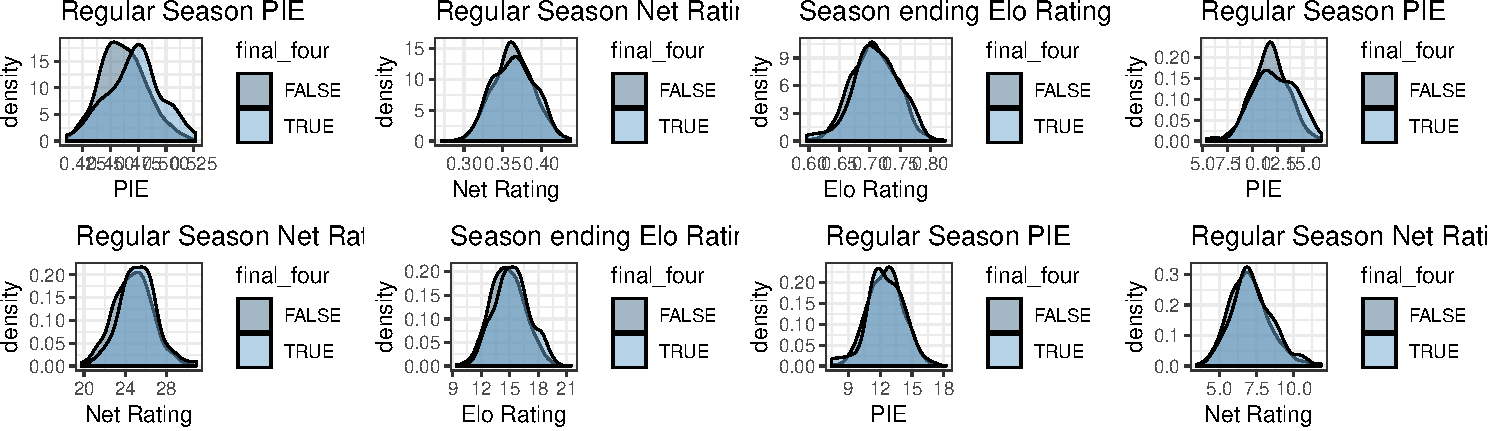
\includegraphics{EDA_files/figure-latex/unnamed-chunk-16-1.pdf}

From the density plots, it actually appears that Final Four teams do
shoot better from the floor during the regular season. Non Final Four
teams shoot around 0.45 during the regular season and Final Four teams
seem to shoot around 0.475. It is very important to keep in mind however
that the sample size for Final Four teams is much smaller than the
sample size for the rest of the tournament field. Therefore its unclear
whether we can consider this difference statistically significant. For
free throw percentage, there does not appear to be much of a difference.

Let's get a better idea of whether the difference in field goal
percentage is real. We can use a two-sample t-test to determine if there
is a difference in the sample means. Because the sample size of the two
are different (and hence the variance), we can use Welch's two-sample
t-test.

\begin{Shaded}
\begin{Highlighting}[]
\NormalTok{fgp_noff <-}\StringTok{ }\NormalTok{stats_season[wins_t, on =}\StringTok{ }\KeywordTok{c}\NormalTok{(}\DataTypeTok{TeamID =} \StringTok{'WTeamID'}\NormalTok{, }\StringTok{'Season'}\NormalTok{), nomatch =}\StringTok{ }\DecValTok{0}
\NormalTok{              ][, final_four }\OperatorTok{:}\ErrorTok{=}\StringTok{ }\NormalTok{tW }\OperatorTok{>=}\StringTok{ }\DecValTok{4}
\NormalTok{                ][final_four }\OperatorTok{==}\StringTok{ }\OtherTok{FALSE}\NormalTok{,  rank_num]}

\NormalTok{fgp_ff <-}\StringTok{ }\NormalTok{stats_season[wins_t, on =}\StringTok{ }\KeywordTok{c}\NormalTok{(}\DataTypeTok{TeamID =} \StringTok{'WTeamID'}\NormalTok{, }\StringTok{'Season'}\NormalTok{), nomatch =}\StringTok{ }\DecValTok{0}
\NormalTok{              ][, final_four }\OperatorTok{:}\ErrorTok{=}\StringTok{ }\NormalTok{tW }\OperatorTok{>=}\StringTok{ }\DecValTok{4}
\NormalTok{                ][final_four }\OperatorTok{==}\StringTok{ }\OtherTok{TRUE}\NormalTok{,  rank_num]}

\KeywordTok{t.test}\NormalTok{(fgp_noff, fgp_ff, }\DataTypeTok{alternative =} \StringTok{'two.sided'}\NormalTok{, }\DataTypeTok{var.equal =} \OtherTok{FALSE}\NormalTok{)}
\end{Highlighting}
\end{Shaded}

\begin{verbatim}
## 
##  Welch Two Sample t-test
## 
## data:  fgp_noff and fgp_ff
## t = 8.1177, df = 102.29, p-value = 1.116e-12
## alternative hypothesis: true difference in means is not equal to 0
## 95 percent confidence interval:
##  2.299050 3.785771
## sample estimates:
## mean of x mean of y 
##  6.042411  3.000000
\end{verbatim}

When doing so, we get a test statistic of -3.1443 and a p-value of
0.002417. At the 95\% significance level therefore, we can reject the
null hypothesis of a zero difference in mean and accept evidence of the
alternative hypothesis that there is a difference in the mean field goal
percentage of Final Four teams and non-Final Four teams. That difference
appears to be about one percentage point.

Now let's do the same thing for rebounding performance.

\begin{Shaded}
\begin{Highlighting}[]
\NormalTok{g1 <-}\StringTok{ }\NormalTok{stats_season[wins_t, on =}\StringTok{ }\KeywordTok{c}\NormalTok{(}\DataTypeTok{TeamID =} \StringTok{'WTeamID'}\NormalTok{, }\StringTok{'Season'}\NormalTok{), nomatch =}\StringTok{ }\DecValTok{0}
\NormalTok{              ][, final_four }\OperatorTok{:}\ErrorTok{=}\StringTok{ }\NormalTok{tW }\OperatorTok{>=}\StringTok{ }\DecValTok{4}\NormalTok{] }\OperatorTok
\StringTok{    }\KeywordTok{ggplot}\NormalTok{(}\KeywordTok{aes}\NormalTok{(}\DataTypeTok{x =}\NormalTok{ DRPG, }\DataTypeTok{y =}\NormalTok{ ORPG, }\DataTypeTok{color =}\NormalTok{ final_four)) }\OperatorTok{+}\StringTok{ }
\StringTok{    }\KeywordTok{geom_point}\NormalTok{(}\DataTypeTok{alpha =} \FloatTok{0.6}\NormalTok{) }\OperatorTok{+}
\StringTok{    }\KeywordTok{labs}\NormalTok{(}
        \DataTypeTok{x =} \StringTok{'Defensive rebounds per game'}\NormalTok{, }
        \DataTypeTok{y =} \StringTok{'Offensive rebounds per game'}\NormalTok{, }
        \DataTypeTok{title =} \StringTok{'Regular Season Rebounding Performance of Tournament Teams'}\NormalTok{) }\OperatorTok{+}
\StringTok{    }\KeywordTok{scale_color_manual}\NormalTok{(}\DataTypeTok{values =} \KeywordTok{c}\NormalTok{(}\StringTok{'darkgrey'}\NormalTok{, }\StringTok{'steelblue'}\NormalTok{)) }

\KeywordTok{ggMarginal}\NormalTok{(g1, }\DataTypeTok{type =} \StringTok{'histogram'}\NormalTok{, }\DataTypeTok{fill =} \StringTok{'steelblue'}\NormalTok{)}
\end{Highlighting}
\end{Shaded}

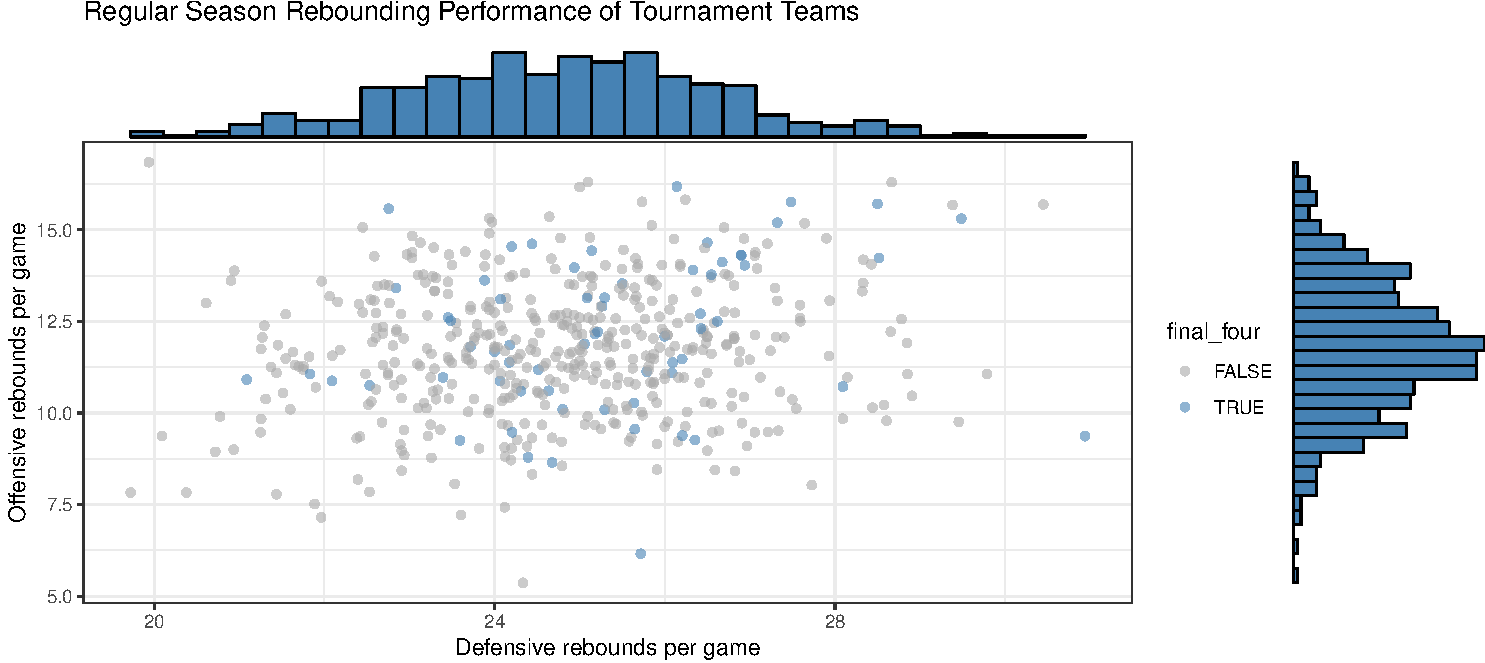
\includegraphics{EDA_files/figure-latex/unnamed-chunk-18-1.pdf}

\begin{Shaded}
\begin{Highlighting}[]
\NormalTok{g1 <-}\StringTok{ }\NormalTok{stats_season[wins_t, on =}\StringTok{ }\KeywordTok{c}\NormalTok{(}\DataTypeTok{TeamID =} \StringTok{'WTeamID'}\NormalTok{, }\StringTok{'Season'}\NormalTok{), nomatch =}\StringTok{ }\DecValTok{0}
\NormalTok{              ][, final_four }\OperatorTok{:}\ErrorTok{=}\StringTok{ }\NormalTok{tW }\OperatorTok{>=}\StringTok{ }\DecValTok{4}\NormalTok{] }\OperatorTok
\StringTok{    }\KeywordTok{ggplot}\NormalTok{(}\KeywordTok{aes}\NormalTok{(}\DataTypeTok{x =}\NormalTok{ DRPG, }\DataTypeTok{fill =}\NormalTok{ final_four)) }\OperatorTok{+}\StringTok{ }
\StringTok{    }\KeywordTok{geom_density}\NormalTok{(}\DataTypeTok{alpha =} \FloatTok{0.6}\NormalTok{) }\OperatorTok{+}\StringTok{ }
\StringTok{    }\KeywordTok{labs}\NormalTok{(}\DataTypeTok{x =} \StringTok{'Defensive rebounds per game'}\NormalTok{, }\DataTypeTok{title =} \StringTok{'Regular Season Rebounding of Tournament Teams'}\NormalTok{)}

\NormalTok{g2 <-}\StringTok{ }\NormalTok{stats_season[wins_t, on =}\StringTok{ }\KeywordTok{c}\NormalTok{(}\DataTypeTok{TeamID =} \StringTok{'WTeamID'}\NormalTok{, }\StringTok{'Season'}\NormalTok{), nomatch =}\StringTok{ }\DecValTok{0}
\NormalTok{              ][, final_four }\OperatorTok{:}\ErrorTok{=}\StringTok{ }\NormalTok{tW }\OperatorTok{>=}\StringTok{ }\DecValTok{4}\NormalTok{] }\OperatorTok
\StringTok{    }\KeywordTok{ggplot}\NormalTok{(}\KeywordTok{aes}\NormalTok{(}\DataTypeTok{x =}\NormalTok{ ORPG, }\DataTypeTok{fill =}\NormalTok{ final_four)) }\OperatorTok{+}\StringTok{ }
\StringTok{    }\KeywordTok{geom_density}\NormalTok{(}\DataTypeTok{alpha =} \FloatTok{0.6}\NormalTok{) }\OperatorTok{+}\StringTok{ }
\StringTok{    }\KeywordTok{labs}\NormalTok{(}\DataTypeTok{x =} \StringTok{'Offensive rebounds per game'}\NormalTok{)}

\KeywordTok{grid.arrange}\NormalTok{(g1, g2, }\DataTypeTok{ncol =} \DecValTok{2}\NormalTok{)}
\end{Highlighting}
\end{Shaded}

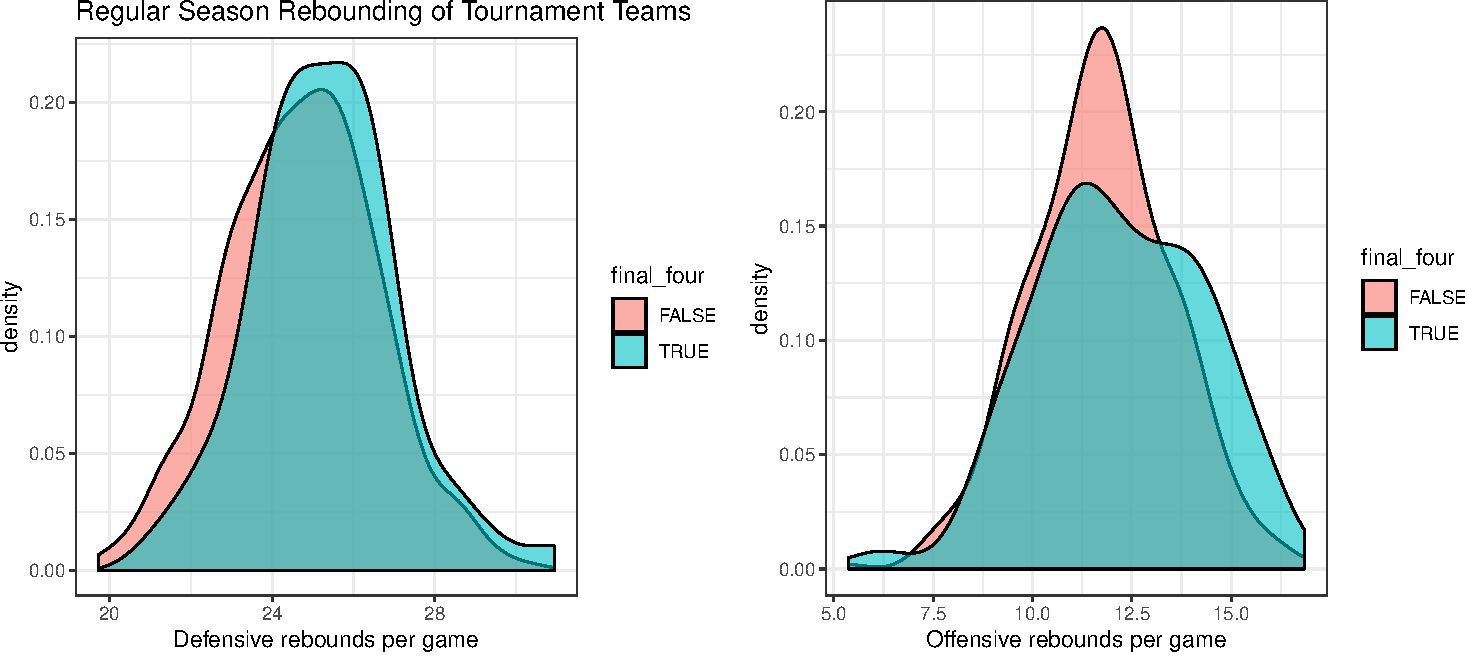
\includegraphics{EDA_files/figure-latex/unnamed-chunk-19-1.pdf}

In terms of defensive rebounding, there does not appear to be much
separation between Final Four teams and the rest of the field. The same
goes for offensive rebounding, however the appears to be a skew in the
distribution for Final Four teams, perhaps an artifact of limited sample
size.

\begin{Shaded}
\begin{Highlighting}[]
\NormalTok{g1 <-}\StringTok{ }\NormalTok{stats_season[wins_t, on =}\StringTok{ }\KeywordTok{c}\NormalTok{(}\DataTypeTok{TeamID =} \StringTok{'WTeamID'}\NormalTok{, }\StringTok{'Season'}\NormalTok{), nomatch =}\StringTok{ }\DecValTok{0}
\NormalTok{              ][, final_four }\OperatorTok{:}\ErrorTok{=}\StringTok{ }\NormalTok{tW }\OperatorTok{>=}\StringTok{ }\DecValTok{4}\NormalTok{] }\OperatorTok
\StringTok{    }\KeywordTok{ggplot}\NormalTok{(}\KeywordTok{aes}\NormalTok{(}\DataTypeTok{x =}\NormalTok{ TOPG, }\DataTypeTok{y =}\NormalTok{ STPG, }\DataTypeTok{color =}\NormalTok{ final_four)) }\OperatorTok{+}\StringTok{ }
\StringTok{    }\KeywordTok{geom_point}\NormalTok{(}\DataTypeTok{alpha =} \FloatTok{0.6}\NormalTok{) }\OperatorTok{+}
\StringTok{    }\KeywordTok{geom_smooth}\NormalTok{(}\KeywordTok{aes}\NormalTok{(}\DataTypeTok{color =}\NormalTok{ final_four), }\DataTypeTok{method =} \StringTok{'lm'}\NormalTok{) }\OperatorTok{+}
\StringTok{    }\KeywordTok{labs}\NormalTok{(}
        \DataTypeTok{x =} \StringTok{'Turnovers per game'}\NormalTok{, }
        \DataTypeTok{y =} \StringTok{'Steals per game'}\NormalTok{, }
        \DataTypeTok{title =} \StringTok{'Turnover Performance of Tournament Teams'}\NormalTok{) }\OperatorTok{+}
\StringTok{    }\KeywordTok{scale_color_manual}\NormalTok{(}\DataTypeTok{values =} \KeywordTok{c}\NormalTok{(}\StringTok{'darkgrey'}\NormalTok{, }\StringTok{'steelblue'}\NormalTok{)) }

\KeywordTok{ggMarginal}\NormalTok{(g1, }\DataTypeTok{type =} \StringTok{'histogram'}\NormalTok{, }\DataTypeTok{fill =} \StringTok{'steelblue'}\NormalTok{)}
\end{Highlighting}
\end{Shaded}

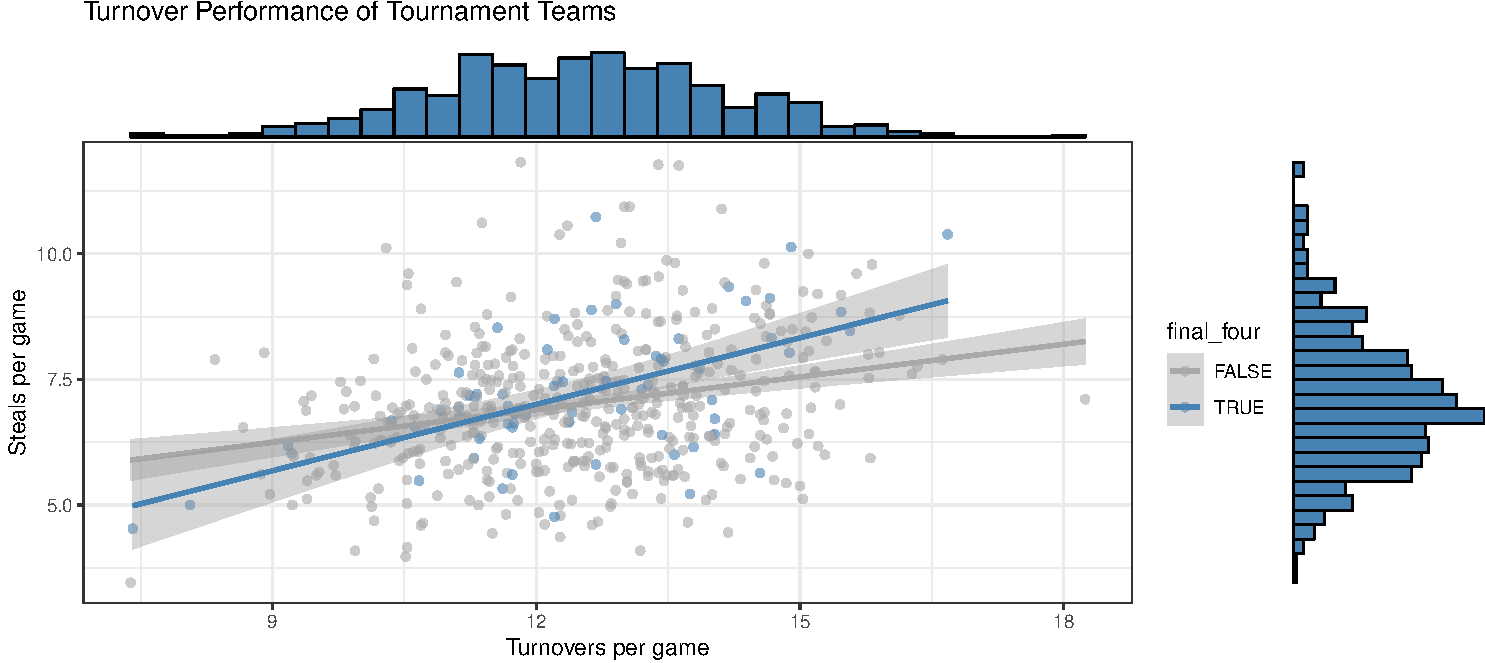
\includegraphics{EDA_files/figure-latex/unnamed-chunk-20-1.pdf}

The ratio of steals to turnovers is positive for all tournament teams,
however the relatioship appears to be stronger for Final Four teams
indicating that this ratio be be a good predictor of tournament success.

\begin{Shaded}
\begin{Highlighting}[]
\NormalTok{g1 <-}\StringTok{ }\NormalTok{stats_season[wins_t, on =}\StringTok{ }\KeywordTok{c}\NormalTok{(}\DataTypeTok{TeamID =} \StringTok{'WTeamID'}\NormalTok{, }\StringTok{'Season'}\NormalTok{), nomatch =}\StringTok{ }\DecValTok{0}
\NormalTok{              ][, final_four }\OperatorTok{:}\ErrorTok{=}\StringTok{ }\NormalTok{tW }\OperatorTok{>=}\StringTok{ }\DecValTok{4}\NormalTok{] }\OperatorTok
\StringTok{    }\KeywordTok{ggplot}\NormalTok{(}\KeywordTok{aes}\NormalTok{(}\DataTypeTok{x =}\NormalTok{ TOPG, }\DataTypeTok{fill =}\NormalTok{ final_four)) }\OperatorTok{+}\StringTok{ }
\StringTok{    }\KeywordTok{geom_density}\NormalTok{(}\DataTypeTok{alpha =} \FloatTok{0.6}\NormalTok{) }\OperatorTok{+}\StringTok{ }
\StringTok{    }\KeywordTok{labs}\NormalTok{(}\DataTypeTok{x =} \StringTok{'Turnovers per game'}\NormalTok{, }\DataTypeTok{title =} \StringTok{'Regular Season Turnovers of Tournament Teams'}\NormalTok{)}

\NormalTok{g2 <-}\StringTok{ }\NormalTok{stats_season[wins_t, on =}\StringTok{ }\KeywordTok{c}\NormalTok{(}\DataTypeTok{TeamID =} \StringTok{'WTeamID'}\NormalTok{, }\StringTok{'Season'}\NormalTok{), nomatch =}\StringTok{ }\DecValTok{0}
\NormalTok{              ][, final_four }\OperatorTok{:}\ErrorTok{=}\StringTok{ }\NormalTok{tW }\OperatorTok{>=}\StringTok{ }\DecValTok{4}\NormalTok{] }\OperatorTok
\StringTok{    }\KeywordTok{ggplot}\NormalTok{(}\KeywordTok{aes}\NormalTok{(}\DataTypeTok{x =}\NormalTok{ STPG, }\DataTypeTok{fill =}\NormalTok{ final_four)) }\OperatorTok{+}\StringTok{ }
\StringTok{    }\KeywordTok{geom_density}\NormalTok{(}\DataTypeTok{alpha =} \FloatTok{0.6}\NormalTok{) }\OperatorTok{+}\StringTok{ }
\StringTok{    }\KeywordTok{labs}\NormalTok{(}\DataTypeTok{x =} \StringTok{'Steals per game'}\NormalTok{,  }\DataTypeTok{title =} \StringTok{'Regular Season Steals of Tournament Teams'}\NormalTok{)}

\KeywordTok{grid.arrange}\NormalTok{(g1, g2, }\DataTypeTok{ncol =} \DecValTok{2}\NormalTok{)}
\end{Highlighting}
\end{Shaded}

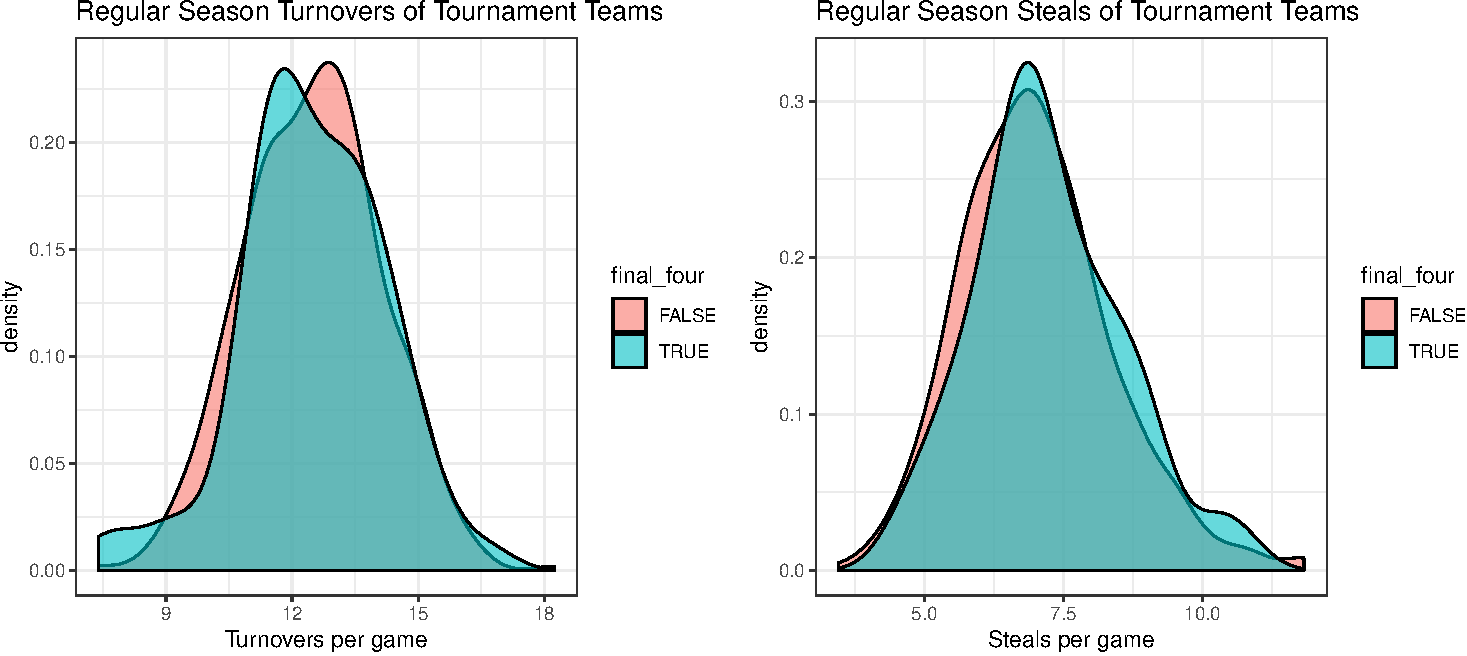
\includegraphics{EDA_files/figure-latex/unnamed-chunk-21-1.pdf}

There seems to be some separation of means between all tournament teams
and Final Four teams for regular season turnovers per game, however its
inconclusive whether or not the difference is significant.

\begin{Shaded}
\begin{Highlighting}[]
\NormalTok{g1 <-}\StringTok{ }\NormalTok{stats_season[wins_t, on =}\StringTok{ }\KeywordTok{c}\NormalTok{(}\DataTypeTok{TeamID =} \StringTok{'WTeamID'}\NormalTok{, }\StringTok{'Season'}\NormalTok{), nomatch =}\StringTok{ }\DecValTok{0}
\NormalTok{              ][, final_four }\OperatorTok{:}\ErrorTok{=}\StringTok{ }\NormalTok{tW }\OperatorTok{>=}\StringTok{ }\DecValTok{4}\NormalTok{] }\OperatorTok
\StringTok{    }\KeywordTok{ggplot}\NormalTok{(}\KeywordTok{aes}\NormalTok{(}\DataTypeTok{x =}\NormalTok{ EFG, }\DataTypeTok{fill =}\NormalTok{ final_four)) }\OperatorTok{+}\StringTok{ }
\StringTok{    }\KeywordTok{geom_density}\NormalTok{(}\DataTypeTok{alpha =} \FloatTok{0.6}\NormalTok{) }\OperatorTok{+}\StringTok{ }
\StringTok{    }\KeywordTok{labs}\NormalTok{(}\DataTypeTok{x =} \StringTok{'Turnovers per game'}\NormalTok{, }\DataTypeTok{title =} \StringTok{'Regular Season Turnovers of Tournament Teams'}\NormalTok{)}


\KeywordTok{grid.arrange}\NormalTok{(g1)}
\end{Highlighting}
\end{Shaded}

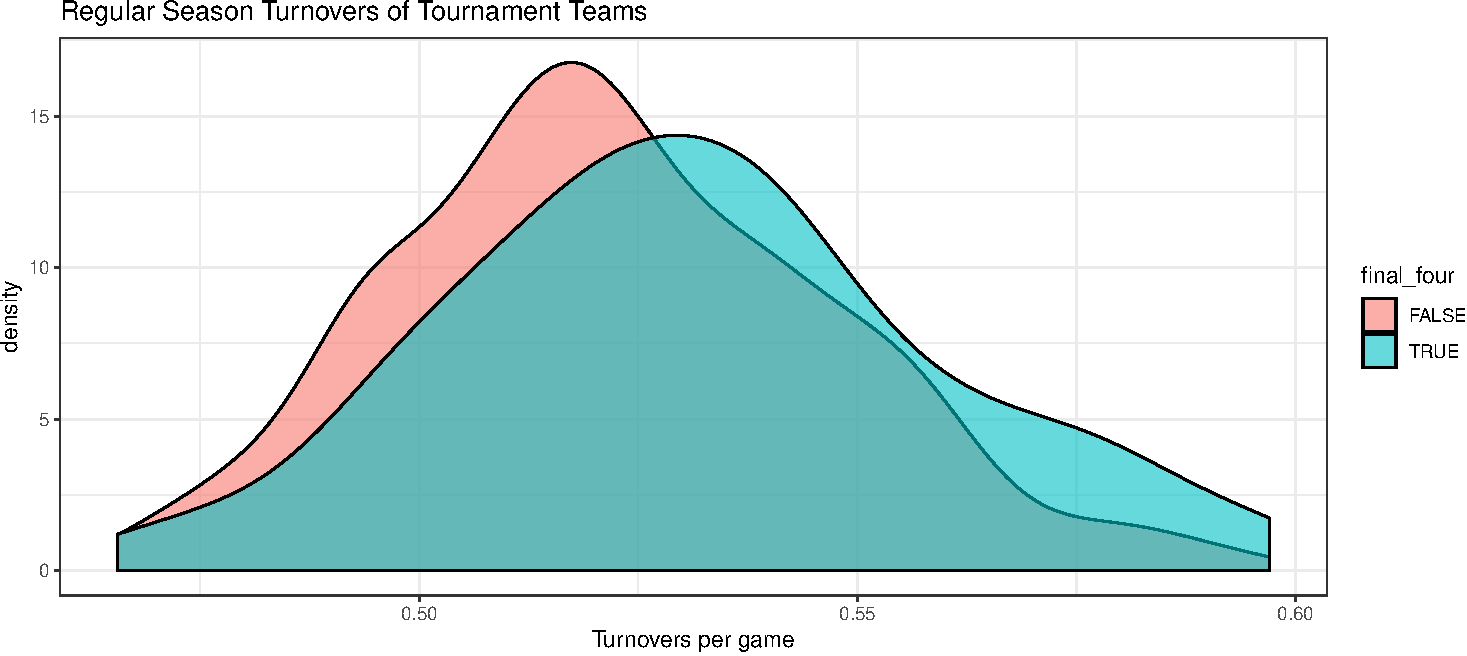
\includegraphics{EDA_files/figure-latex/unnamed-chunk-22-1.pdf}


\end{document}
